\documentclass[aspectratio=169,10pt]{beamer}

\usetheme{Madrid}
\usecolortheme{seahorse}

\usepackage{amsmath,amssymb,amsfonts}
\usepackage{bm}
\usepackage{graphicx}
\usepackage{booktabs}
\usepackage{listings}
\usepackage{xcolor}
\usepackage{tikz}
\usepackage{array}
\usepackage{microtype}

\graphicspath{{figures/}}

\lstdefinestyle{python}{
  language=Python,
  basicstyle=\ttfamily\scriptsize,
  numbers=left,
  numberstyle=\tiny\color{gray},
  frame=single,
  backgroundcolor=\color{gray!7},
  keywordstyle=\color{blue!70!black}\bfseries,
  commentstyle=\color{green!50!black}\itshape,
  stringstyle=\color{orange!80!black},
  showstringspaces=false,
  breaklines=true,
  tabsize=4,
}

\setbeamertemplate{footline}[frame number]
\setbeamertemplate{navigation symbols}{}

% ── title page ──────────────────────────────────────────────────────────────
\title[Ch.\ 24: Multidisciplinary Optimization]{Chapter 24:\\Multidisciplinary Optimization}
\subtitle{\textit{Algorithms for Optimization}, 2nd ed.\ (2026)\\
Kochenderfer \& Wheeler}
\author{Lecture Notes}
\date{\today}

\begin{document}

\begin{frame}
  \titlepage
\end{frame}

% ── outline ─────────────────────────────────────────────────────────────────
\begin{frame}{Chapter Outline}
  \tableofcontents
\end{frame}

% ============================================================================
\section{Introduction to Multidisciplinary Design Optimization}
% ============================================================================

\begin{frame}[allowframebreaks]{What is Multidisciplinary Design Optimization?}

  Real engineering systems --- aircraft, autonomous vehicles, power grids,
  financial portfolios --- are not designed one component at a time.
  Every component interacts with every other component, and the best choice
  for one discipline (say, the lightest wing structure) may be terrible for
  another (e.g., aerodynamic performance demands a thicker profile).
  \textbf{Multidisciplinary Design Optimization (MDO)} is the branch of
  optimization that takes all of these interactions seriously and seeks a
  system-level optimum rather than a collection of local discipline optima.

  \begin{block}{What Makes MDO Different from Ordinary Optimization}
    In a single-discipline problem you minimize $f(\mathbf{x})$ subject to
    constraints on $\mathbf{x}$ (x, the vector of design variables).
    In an MDO problem the objective depends on \emph{outputs} of several
    interacting analyses, and each analysis may depend on outputs of the
    others.  This circular dependency is the central challenge.
  \end{block}

  \medskip
  The most important consequence of these interdependencies is that
  optimizing each discipline in isolation --- first optimize the structure,
  then optimize the aerodynamics, and so on --- generally does \emph{not}
  produce the system-level optimum.  The disciplines must be considered
  simultaneously.

  \begin{exampleblock}{Everyday Analogy}
    Imagine co-designing a backpack and a bicycle: the backpack should be
    as small as possible, but its size affects the rider's aerodynamic drag,
    which in turn affects what gear ratio is optimal for the bicycle, which
    feeds back into how heavy the bicycle can be, which determines how the
    backpack should be attached.  Every dimension affects every other;
    no single dimension can be optimized independently.
  \end{exampleblock}

  \framebreak

  \begin{columns}[T]
    \column{0.55\textwidth}
    \textbf{Core challenges in MDO:}

    \medskip
    \textit{Circular dependencies.}  Discipline A needs outputs from
    Discipline B, which needs outputs from Discipline A.  This creates a
    system of equations that must be solved simultaneously, not sequentially.

    \medskip
    \textit{Heterogeneous solvers.}  Different disciplines are often owned by
    different teams and use different software (finite-element codes,
    computational-fluid-dynamics solvers, market-simulation tools).  The MDO
    architecture must orchestrate these without rewriting them.

    \medskip
    \textit{Expensive function evaluations.}  A single call to a
    high-fidelity CFD or FEA solver can take hours.  The MDO architecture
    must therefore minimise the number of such calls.

    \medskip
    \textit{Large variable counts.}  Even simple systems have dozens of
    design variables per discipline; the combined problem can have thousands.

    \column{0.42\textwidth}
    \begin{center}
      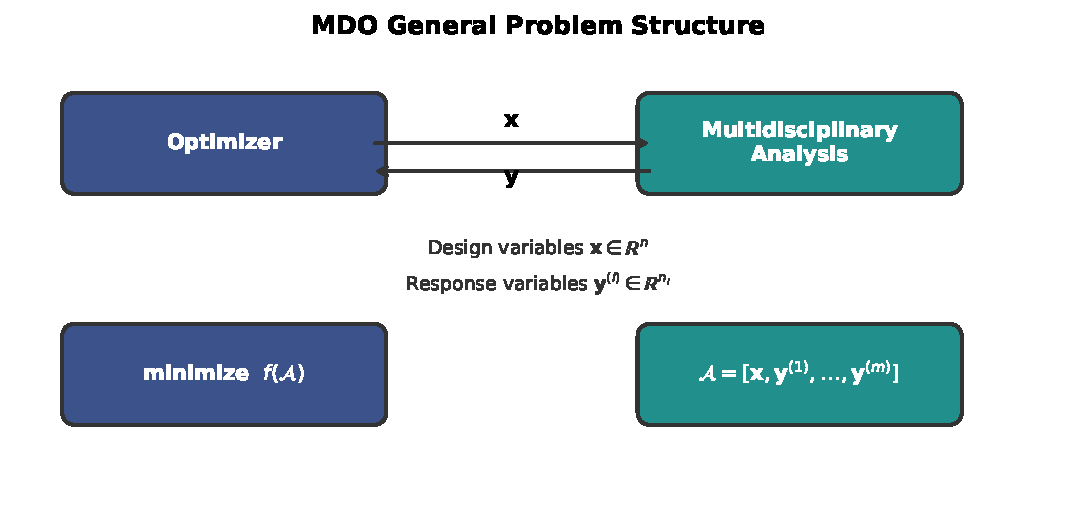
\includegraphics[width=\textwidth]{fig_mdo_structure.pdf}
    \end{center}
    \begin{block}{General MDO Problem Statement}
      \[
        \min_{\mathcal{A}}\; f(\mathcal{A})
        \quad \text{subject to} \quad
        \mathcal{F}_i(\mathcal{A}) = \mathcal{A},\;\forall\, i
      \]
      where $\mathcal{A}$ (the \emph{assignment}) collects all design and
      response variables, and the constraints say that running every
      disciplinary analysis $\mathcal{F}_i$ (script F sub $i$) must leave
      the assignment unchanged.
    \end{block}
  \end{columns}

  \begin{alertblock}{Key Insight}
    The feasibility condition $\mathcal{F}_i(\mathcal{A})=\mathcal{A}$ is
    simply a mathematical way of saying ``the disciplines agree with each
    other.''  Finding such an assignment --- let alone the best one --- is
    what MDO architectures are designed to accomplish.
  \end{alertblock}

\end{frame}

% ============================================================================
\section{Disciplinary Analyses and Assignments}
% ============================================================================

\begin{frame}[allowframebreaks]{Disciplinary Analyses}

  To describe MDO precisely, we need two foundational concepts: the
  \emph{assignment} and the \emph{disciplinary analysis}.

  \begin{block}{Definition: Assignment $\mathcal{A}$}
    An \textbf{assignment} $\mathcal{A}$ is a dictionary (a mapping from
    variable names to numerical values) that records the current values of
    \emph{all} variables in the system: the design variables $\mathbf{x}$
    (the quantities we are free to choose) and the response variables
    $\mathbf{y}^{(1)}, \ldots, \mathbf{y}^{(m)}$ (quantities computed by
    each of the $m$ disciplines).  The total size of the assignment is
    $|\mathcal{A}| = n + \sum_{i=1}^{m} n_i$, where $n$ is the number of
    design variables and $n_i$ (n sub $i$) is the number of response
    variables produced by discipline $i$.
  \end{block}

  \begin{block}{Definition: Disciplinary Analysis $\mathcal{F}_i$}
    A \textbf{disciplinary analysis} $\mathcal{F}_i$ (script F sub $i$) is
    a function that reads the current assignment and updates (overwrites)
    the response variables of discipline $i$:
    \[
      \mathbf{y}^{(i)} \;\leftarrow\; \mathcal{F}_i\!\left(\mathbf{x},\;
      \mathbf{y}^{(-i)}\right)
    \]
    where $\mathbf{y}^{(-i)}$ (y superscript minus $i$) denotes all
    response variables \emph{except} those of discipline $i$.  In practice
    $\mathcal{F}_i$ is often a black-box simulation (a finite-element solver,
    a routing algorithm, a pricing model, \ldots).
  \end{block}

  \medskip
  The arrow $\leftarrow$ means ``is assigned the value of''.  After running
  $\mathcal{F}_i$, the variable $\mathbf{y}^{(i)}$ in the shared assignment
  dictionary holds the new, updated value.

  \framebreak

  \begin{exampleblock}{Example 24.1: Three-Discipline System}
    Consider a system with one design variable $x$ and three disciplines,
    each producing one response variable:
    \begin{align*}
      y^{(1)} &\leftarrow \mathcal{F}_1\!\left(x, y^{(2)}, y^{(3)}\right)
               = y^{(2)} - x \\
      y^{(2)} &\leftarrow \mathcal{F}_2\!\left(x, y^{(1)}, y^{(3)}\right)
               = \sin\!\bigl(y^{(1)} + y^{(3)}\bigr) \\
      y^{(3)} &\leftarrow \mathcal{F}_3\!\left(x, y^{(1)}, y^{(2)}\right)
               = \cos\!\bigl(x + y^{(1)} + y^{(2)}\bigr)
    \end{align*}
    Notice that $\mathcal{F}_1$ needs $y^{(2)}$, $\mathcal{F}_2$ needs
    $y^{(1)}$ and $y^{(3)}$, and $\mathcal{F}_3$ needs $y^{(1)}$ and
    $y^{(2)}$.  These are \emph{circular} dependencies: no discipline can
    be run ``first'' without some assumption about the others.
  \end{exampleblock}

  \medskip
  \textbf{What this means concretely.}  Suppose we start with the initial
  guess $x=1$, $y^{(1)}=y^{(2)}=y^{(3)}=1$.  Running $\mathcal{F}_1$
  gives $y^{(1)} = 1 - 1 = 0$.  Running $\mathcal{F}_2$ then gives
  $y^{(2)} = \sin(0 + 1) \approx 0.841$.  Running $\mathcal{F}_3$ gives
  $y^{(3)} = \cos(1 + 0 + 0.841) \approx -0.297$.  We are not done: the
  new $y^{(3)}$ would change $y^{(2)}$, which would change $y^{(1)}$, and
  so on.  We must iterate until all three disciplines agree simultaneously.

  \begin{alertblock}{Key Insight}
    A disciplinary analysis is a function, not a solve.  It takes the
    current state of the whole system (the assignment) and returns a
    \emph{new} value for its own outputs.  The challenge is to find an
    assignment where running any analysis leaves the assignment unchanged
    --- the concept of \emph{interdisciplinary compatibility}.
  \end{alertblock}

\end{frame}

\begin{frame}[fragile]{Python: Implementing Disciplinary Analyses (Example 24.1)}

  The simplest way to implement disciplinary analyses in Python is to
  represent the assignment as a dictionary and have each analysis function
  mutate the relevant entries in place.

  \begin{lstlisting}[style=python]
import numpy as np

# Each disciplinary analysis takes the shared assignment dict,
# reads what it needs, and writes its own response variables.

def F1(A):
    """Discipline 1: y^(1) = y^(2) - x."""
    A['y1'] = A['y2'] - A['x']
    return A

def F2(A):
    """Discipline 2: y^(2) = sin(y^(1) + y^(3))."""
    A['y2'] = np.sin(A['y1'] + A['y3'])
    return A

def F3(A):
    """Discipline 3: y^(3) = cos(x + y^(1) + y^(2))."""
    A['y3'] = np.cos(A['x'] + A['y2'] + A['y1'])
    return A

# ── initial assignment for x = 1, all response vars = 1 ──────────────────
A = {'x': 1.0, 'y1': 1.0, 'y2': 1.0, 'y3': 1.0}

# ── run one pass in the ordering F1, F2, F3 ──────────────────────────────
A = F1(A); A = F2(A); A = F3(A)
print(A)
# {'x': 1.0, 'y1': 0.0, 'y2': 0.8415, 'y3': -0.2972}  (first iteration only)
  \end{lstlisting}

  \begin{columns}[T]
    \column{0.50\textwidth}
    \begin{block}{What the Code Shows}
      After a single pass the values have changed, but they have not
      converged to a fixed point yet.  Each function reads whatever values
      are currently in \texttt{A} when it runs, so the ordering of calls
      matters: if $F_3$ runs before $F_2$, it reads a stale $y^{(2)}$.
      This is why the ordering of analyses is a design decision in MDO.
    \end{block}

    \column{0.47\textwidth}
    \begin{block}{Circular Dependencies}
      \[
        \mathcal{F}_1 \;\text{needs}\; y^{(2)},
        \quad
        \mathcal{F}_2 \;\text{needs}\; y^{(1)}, y^{(3)},
        \quad
        \mathcal{F}_3 \;\text{needs}\; y^{(1)}, y^{(2)}
      \]
      Every discipline feeds into at least one other discipline,
      forming a cycle: $\mathcal{F}_1 \to \mathcal{F}_2 \to
      \mathcal{F}_3 \to \mathcal{F}_1$.
    \end{block}
  \end{columns}

\end{frame}

% ============================================================================
\section{Interdisciplinary Compatibility and the MDA}
% ============================================================================

\begin{frame}[allowframebreaks]{Interdisciplinary Compatibility}

  We now give a precise definition of what it means for an assignment to be
  \emph{self-consistent}, i.e., for all disciplines to agree with one another.

  \begin{block}{Definition: Interdisciplinary Compatibility}
    An assignment $\mathcal{A}$ is called \textbf{interdisciplinarily
    compatible} (or simply \emph{feasible}) if running every disciplinary
    analysis leaves the assignment unchanged:
    \[
      \mathcal{F}_i(\mathcal{A}) = \mathcal{A}
      \quad \text{for all } i = 1, \ldots, m
    \]
    Equivalently, the \emph{disciplinary residual}
    $R_i(\mathcal{A}) \equiv \mathcal{F}_i(\mathcal{A}) - \mathcal{A}$
    equals zero for every discipline $i$.  Here ``R'' stands for residual:
    the amount by which the discipline's output \emph{differs} from what is
    currently stored in the assignment.
  \end{block}

  \medskip
  A compatible assignment is the analogue of a fixed point of the system of
  equations.  At such a point, if you ask any discipline ``given the current
  values of everything else, what would you compute for your own outputs?''
  it answers with the values already stored in the assignment.  There is no
  more updating to do.

  \medskip
  To find a compatible assignment we use a process called a
  \textbf{Multidisciplinary Analysis (MDA)}, which is simply an iterative
  algorithm that keeps running the disciplinary analyses in turn until
  they stop changing the assignment.

  \framebreak

  \begin{columns}[T]
    \column{0.50\textwidth}
    \begin{block}{Dependency Graphs}
      The interaction structure of a multidisciplinary system is best
      visualised as a \textbf{directed graph}, where:
      \begin{itemize}
        \item Each node represents a discipline (or a variable).
        \item A directed edge $i \to j$ means ``discipline $j$
              requires the output of discipline $i$.''
      \end{itemize}
      If the graph has \textbf{no cycles}, the analyses can be run in
      topological order (a sequence where each discipline's inputs are
      already available) and the system is solved in a single pass.
      If the graph has \textbf{cycles}, iterative solution (an MDA) is
      unavoidable.
    \end{block}

    \medskip
    Topological sorting is a standard graph algorithm that, given a
    directed acyclic graph (DAG), produces a linear ordering of the nodes
    such that every edge points ``forward'' in the ordering.  For an MDO
    dependency graph with no cycles, running the analyses in topological
    order guarantees a single-pass solve.

    \column{0.47\textwidth}
    \begin{center}
      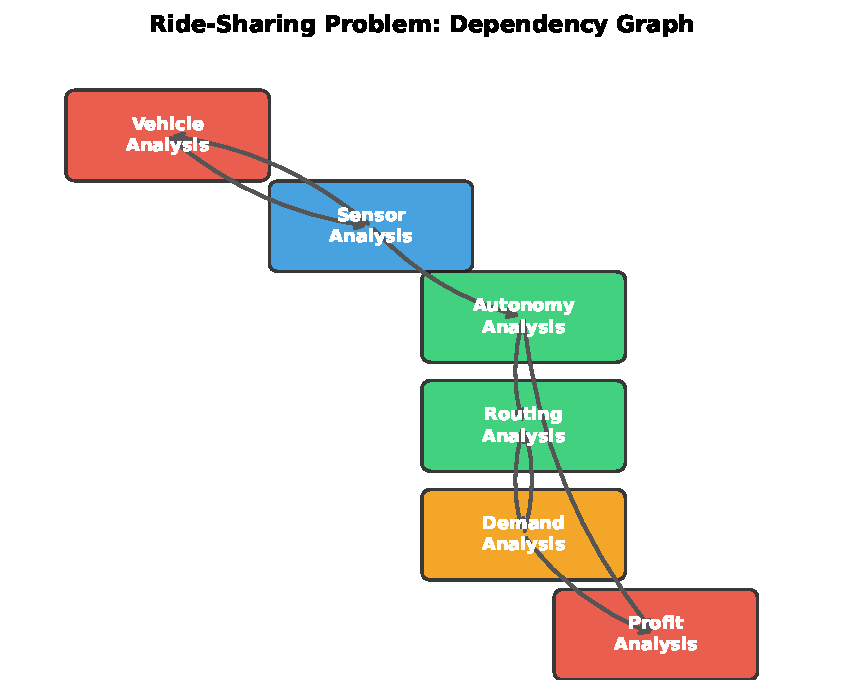
\includegraphics[width=0.9\textwidth]{fig_dependency_graph.pdf}\\
      \small Dependency graph for the ride-sharing problem (introduced
      later).  The two-way arrows between Vehicle and Sensor, and between
      Routing and Demand, indicate cycles that require iterative solution.
    \end{center}
  \end{columns}

  \begin{alertblock}{Key Insight}
    Before choosing an MDO architecture, always draw the dependency graph.
    If there are no cycles (rare in complex engineering systems) a single
    forward pass suffices.  If there are cycles, the choice of
    architecture determines how those cycles are resolved --- and that
    choice has major implications for computational cost.
  \end{alertblock}

\end{frame}

\begin{frame}[allowframebreaks]{The Gauss-Seidel MDA Algorithm}

  The simplest and most widely used iterative MDA algorithm is the
  \textbf{Gauss-Seidel} (pronounced ``gows-ZY-del'') method, named after
  the same iterative scheme used to solve systems of linear equations.
  The idea is straightforward: cycle through the disciplinary analyses
  repeatedly, each time updating the assignment with the latest values,
  until the assignment stops changing.

  \begin{block}{Algorithm 24.1: Gauss-Seidel MDA}
    \textbf{Inputs:}
    \begin{itemize}
      \item $[F_1, \ldots, F_m]$ --- the list of disciplinary analysis
            functions, in the desired evaluation order.
      \item $\mathcal{A}$ --- an initial assignment (an initial guess for
            all response variables; the design variable $\mathbf{x}$ is
            fixed for this call).
      \item $k_{\max}$ --- the maximum number of outer iterations (a
            safeguard against infinite loops if the system does not converge).
      \item $\varepsilon$ (epsilon) --- the relative convergence tolerance:
            we declare convergence when no variable changes by more than a
            fraction $\varepsilon$ of its current magnitude.
    \end{itemize}
    \textbf{Procedure:}
    \begin{enumerate}
      \item Set $k \leftarrow 0$, \texttt{converged} $\leftarrow$
            \texttt{False}.
      \item While not converged and $k \leq k_{\max}$:
        \begin{enumerate}
          \item $k \leftarrow k + 1$.
          \item Save a deep copy: $\mathcal{A}_{\text{old}} \leftarrow
                \mathcal{A}$.
          \item For each discipline $F_i$ in order: run $F_i(\mathcal{A})$,
                updating $\mathcal{A}$ in place.
          \item Check: set \texttt{converged} $=$ \texttt{True} if
                $|v(\mathcal{A}) - v(\mathcal{A}_{\text{old}})| \leq
                \varepsilon \cdot |v(\mathcal{A}_{\text{old}})|$ for
                every numeric variable $v$.
        \end{enumerate}
      \item Return $(\mathcal{A},\; \texttt{converged})$.
    \end{enumerate}
  \end{block}

  \framebreak

  \begin{columns}[T]
    \column{0.50\textwidth}
    \textbf{Why ordering matters.}  The Gauss-Seidel method uses the most
    recently updated value of each variable in subsequent analyses within
    the same outer iteration.  This means that if $\mathcal{F}_2$ runs
    after $\mathcal{F}_1$, it uses the freshly updated $y^{(1)}$, which
    tends to propagate information faster and improves convergence.

    \medskip
    For an acyclic graph, the optimal ordering is the \textbf{topological
    sort}: run analyses in the order imposed by the dependency graph, so
    that each analysis receives fully up-to-date inputs.  For a cyclic
    graph, there is no perfect ordering, but a topological sort applied to
    a \emph{strongly connected component} (the subset of nodes in a cycle)
    can still reduce the number of ``stale'' inputs and thereby speed up
    convergence.

    \medskip
    \begin{alertblock}{Example 24.2: Ordering Effect}
      For the three-discipline system with $x=1$, starting at all-ones:
      ordering $F_1, F_2, F_3$ converges in roughly 15 iterations.
      Ordering $F_1, F_3, F_2$ \emph{oscillates and does not converge}.
      The only difference is the order of two function calls.
    \end{alertblock}

    \column{0.48\textwidth}
    \begin{center}
      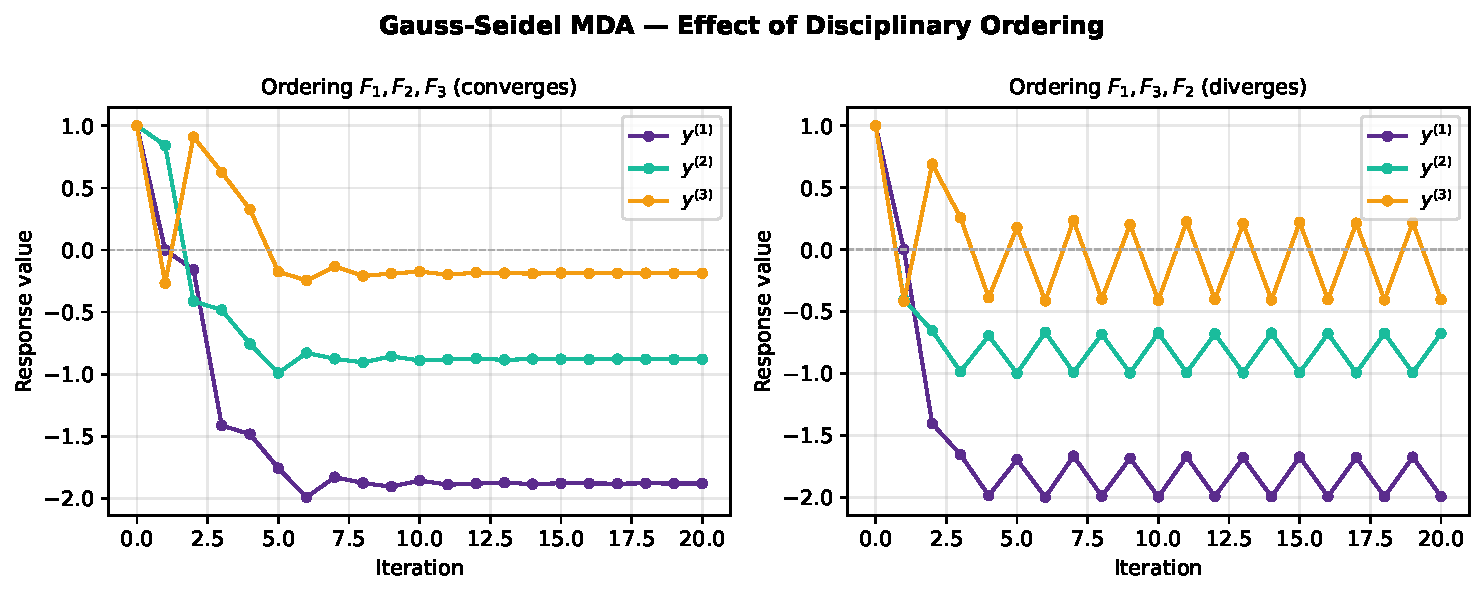
\includegraphics[width=\textwidth]{fig_gauss_seidel.pdf}\\
      \small Top: ordering $F_1,F_2,F_3$ converges.
      Bottom: ordering $F_1,F_3,F_2$ oscillates indefinitely.
      Both plots show $y^{(1)}$ (purple), $y^{(2)}$ (teal),
      $y^{(3)}$ (green) vs.\ iteration number.
    \end{center}
  \end{columns}

  \medskip
  \textbf{Convergence rate.}  The Gauss-Seidel MDA converges when the
  spectral radius (the magnitude of the largest eigenvalue) of the
  Jacobian $\partial \mathbf{y} / \partial \mathbf{y}$ evaluated at the
  fixed point is less than one.  ``Spectral radius'' here measures how
  strongly disciplines amplify perturbations in one another's outputs.
  A radius near zero means fast convergence; a radius near one means slow
  convergence; a radius above one means divergence.

\end{frame}

\begin{frame}[fragile]{Python: Gauss-Seidel MDA Implementation}

  The Python implementation below closely follows Algorithm 24.1.
  It works with any list of disciplinary analysis functions as long as
  each function accepts and mutates the shared assignment dictionary.

  \begin{lstlisting}[style=python]
import copy, numpy as np

def gauss_seidel_mda(Fs, A, k_max=100, eps=1e-6):
    """
    Run the Gauss-Seidel MDA until convergence or k_max iterations.

    Parameters
    ----------
    Fs     : list of callables, each of the form F(A) -> A (mutates in place)
    A      : dict, the shared assignment {'x': ..., 'y1': ..., ...}
    k_max  : int, maximum number of outer iterations
    eps    : float (epsilon), relative convergence tolerance

    Returns
    -------
    A          : dict, the (hopefully converged) assignment
    converged  : bool, True iff the tolerance was met
    """
    k, converged = 0, False
    while not converged and k <= k_max:
        k += 1
        A_old = copy.deepcopy(A)     # save a snapshot before this iteration
        for F in Fs:
            F(A)                     # each analysis updates A in place
        # Check whether every numeric variable changed by less than eps
        converged = all(
            abs(A[v] - A_old[v]) <= eps * (abs(A_old[v]) + 1e-12)
            for v in A if isinstance(A[v], (int, float, np.floating))
        )
    return A, converged

# ── Apply to Example 24.2 with the converging ordering ───────────────────
A = {'x': 1.0, 'y1': 1.0, 'y2': 1.0, 'y3': 1.0}
A_sol, ok = gauss_seidel_mda([F1, F2, F3], A, k_max=200, eps=1e-8)
print(f"Converged: {ok}")
print(f"y1 = {A_sol['y1']:.6f}")
print(f"y2 = {A_sol['y2']:.6f}")
print(f"y3 = {A_sol['y3']:.6f}")
# Converged: True
# y1 = -1.243698   y2 = -0.243698   y3 = -0.219571
  \end{lstlisting}

  \begin{block}{Interpretation of the Output}
    At the converged assignment with $x=1$, we have
    $y^{(1)} \approx -1.244$, $y^{(2)} \approx -0.244$,
    $y^{(3)} \approx -0.220$.  You can verify by hand: $y^{(2)} - x
    = -0.244 - 1 = -1.244 = y^{(1)}$ (check!), and
    $\sin(y^{(1)} + y^{(3)}) = \sin(-1.244 - 0.220) \approx -0.244 = y^{(2)}$
    (check!).  The system is consistent.
  \end{block}

\end{frame}

% ============================================================================
\section{MDO Architectures: Overview and the Running Example}
% ============================================================================

\begin{frame}[allowframebreaks]{MDO Architectures: Overview}

  Having defined what it means for an assignment to be feasible
  (interdisciplinarily compatible) and how to find such an assignment via
  the MDA, we now turn to the central question of this chapter:
  \emph{how should the MDA be embedded inside an optimizer?}

  Different answers to this question give rise to different
  \textbf{MDO architectures}.  Each architecture is a blueprint that
  specifies:
  \begin{enumerate}
    \item Which variables are optimiser decision variables (the things the
          optimiser directly controls).
    \item How and when the disciplinary analyses are called.
    \item How coupling between disciplines is enforced (either through
          an inner MDA loop, through equality constraints, or through
          a bi-level structure).
  \end{enumerate}

  \begin{block}{The General MDO Problem}
    All architectures solve, in one form or another, the same underlying
    problem:
    \[
      \min_{\mathcal{A}} f(\mathcal{A})
      \quad \text{subject to} \quad
      \mathcal{F}_i(\mathcal{A}) = \mathcal{A},\; i=1,\ldots,m,
      \quad \mathcal{A} \in \mathcal{X}
    \]
    where $f$ (f) is the system-level objective (e.g., negative profit,
    total weight, total cost), $\mathcal{F}_i$ are the disciplinary
    analyses, and $\mathcal{X}$ encodes bounds and inequality constraints
    on the design and response variables.
  \end{block}

  \framebreak

  \begin{center}
    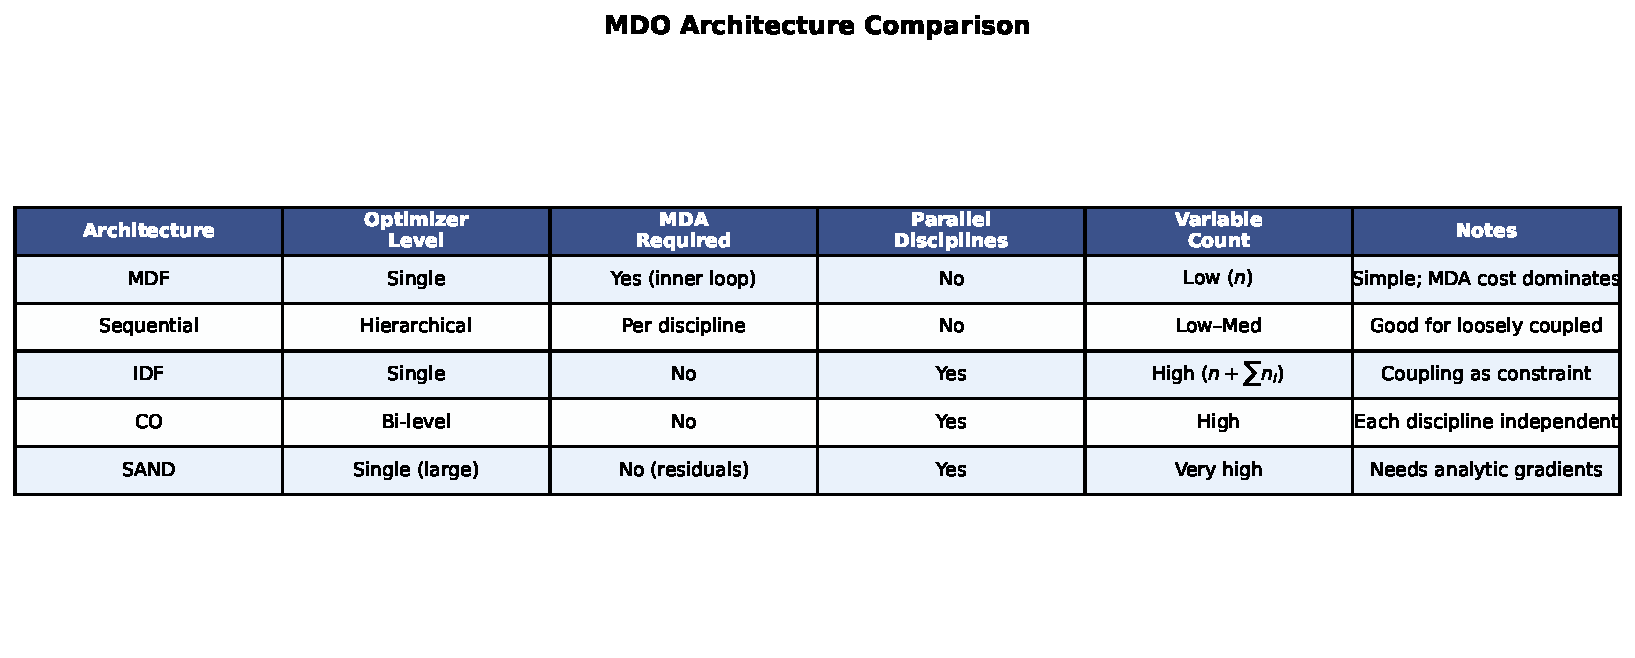
\includegraphics[width=0.75\textwidth]{fig_architecture_comparison.pdf}
  \end{center}

  This chapter covers five main architectures, each making a different
  trade-off between these factors:

  \begin{columns}[T]
    \column{0.48\textwidth}
    \textbf{Single-level architectures} use one optimizer that directly
    controls the outcome:
    \begin{itemize}
      \item \textbf{Multidisciplinary Design Feasible (MDF)}: the simplest
            approach; every function evaluation runs a full MDA.
      \item \textbf{Individual Discipline Feasible (IDF)}: no MDA loop;
            coupling enforced via equality constraints.
      \item \textbf{Simultaneous Analysis and Design (SAND)}: the most
            direct formulation; analysis residuals are explicit constraints.
    \end{itemize}

    \column{0.48\textwidth}
    \textbf{Hierarchical / distributed architectures} split the problem
    across multiple levels or teams:
    \begin{itemize}
      \item \textbf{Sequential Optimization}: disciplines optimise one
            after another in a round-robin fashion.
      \item \textbf{Collaborative Optimization (CO)}: each discipline has
            its own sub-optimizer; a system-level optimizer coordinates.
    \end{itemize}
  \end{columns}

\end{frame}

\begin{frame}[allowframebreaks]{Running Example: The Ride-Sharing Company (Example 24.3)}

  To make the comparison between architectures concrete, the textbook uses
  a single running example throughout the chapter: a hypothetical
  autonomous ride-sharing company that is \emph{simultaneously} designing
  several interacting components of its business.

  \begin{columns}[T]
    \column{0.55\textwidth}
    \textbf{The four design vectors:}
    \begin{itemize}
      \item $\mathbf{v}$ (vehicle): structural geometry, engine and drive
            train, battery capacity, passenger capacity, weight, drag.
      \item $\mathbf{s}$ (sensor package): the autonomous driving sensors
            (cameras, lidar, radar); must meet safety requirements that
            depend on the vehicle geometry.
      \item $\mathbf{r}$ (routing strategy): the algorithm that dispatches
            vehicles to passenger requests; performance depends on vehicle
            range and the number of simultaneous passengers.
      \item $\mathbf{p}$ (pricing scheme): the fare structure; affects
            passenger demand, which in turn affects routing performance.
    \end{itemize}

    \medskip
    \textbf{The objective}: maximise profit (equivalently, minimise
    negative profit), where profit is a function of all of the above plus
    the outcomes of the disciplinary analyses.

    \column{0.43\textwidth}
    \begin{center}
      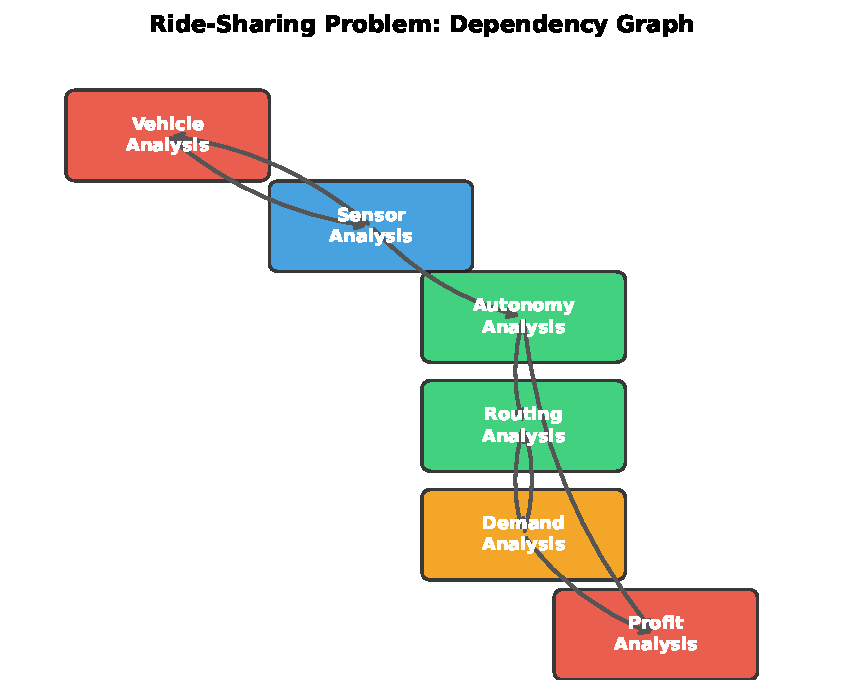
\includegraphics[width=\textwidth]{fig_dependency_graph.pdf}
    \end{center}
    \small
    The dependency diagram shows the six analyses and their couplings.
    Two cycles are present:
    (1) Vehicle $\leftrightarrow$ Sensor (tight coupling: vehicle geometry
    determines sensor requirements; sensor weight affects vehicle
    performance).
    (2) Routing $\leftrightarrow$ Demand (tight coupling: routing
    performance affects demand; demand level affects routing).
  \end{columns}

  \framebreak

  \textbf{The six disciplinary analyses:}
  \begin{enumerate}
    \item \textbf{Vehicle Analysis}: given $\mathbf{v}$ and sensor weight
          from the sensor analysis, computes vehicle range, fuel efficiency,
          and weight.
    \item \textbf{Sensor Analysis}: given vehicle geometry and performance
          from the vehicle analysis, computes sensor specifications and
          sensor weight.
    \item \textbf{Autonomy Analysis}: given vehicle and sensor outputs,
          evaluates the autonomy level (how capable the self-driving system
          is under various conditions).
    \item \textbf{Routing Analysis}: given autonomy level and passenger
          demand from the demand analysis, computes routing performance
          (average wait time, throughput).
    \item \textbf{Demand Analysis}: given routing performance and the
          pricing scheme, estimates passenger demand.
    \item \textbf{Profit Analysis}: given all other outputs plus vehicle and
          pricing design variables, computes net profit.
  \end{enumerate}

  \begin{alertblock}{Why This Example is Challenging}
    The two cycles (Vehicle$\leftrightarrow$Sensor and
    Routing$\leftrightarrow$Demand) mean a full MDA is needed at every
    point evaluated.  Each architecture handles these cycles differently,
    with different implications for how many times each analysis is called
    and what is left for the optimizer to control.
  \end{alertblock}

\end{frame}

% ============================================================================
\section{Multidisciplinary Design Feasible (MDF)}
% ============================================================================

\begin{frame}[allowframebreaks]{MDF: Multidisciplinary Design Feasible Architecture}

  The \textbf{Multidisciplinary Design Feasible (MDF)} architecture is
  conceptually the simplest of all MDO architectures.  Its central idea
  is to hide all the complexity of the coupled system \emph{inside} a
  black-box function that the optimizer sees as an ordinary, single-discipline
  objective function.

  \textbf{The key idea.}  At every point $\mathbf{x}$ that the optimizer
  proposes, MDF runs a complete inner MDA loop (e.g., Gauss-Seidel) to
  find the unique compatible assignment $\mathcal{A}^*(\mathbf{x})$ such
  that all disciplines agree.  Only once this inner convergence is achieved
  is the objective $f(\mathcal{A}^*(\mathbf{x}))$ returned to the optimizer.

  \begin{block}{MDF Problem Formulation}
    From the optimizer's perspective, MDF solves:
    \[
      \min_{\mathbf{x} \in \mathcal{X}}\;
      f\!\bigl(\mathrm{MDA}(\mathbf{x})\bigr)
    \]
    where $\mathrm{MDA}(\mathbf{x})$ (MDA stands for Multidisciplinary
    Analysis) is a function that, given design variables $\mathbf{x}$,
    runs the iterative Gauss-Seidel loop until convergence and returns
    the fully compatible assignment $\mathcal{A}^*$.  The optimizer only
    sees a function of $\mathbf{x}$ and has no knowledge of the inner
    iteration; it treats MDA as a black-box simulation.
  \end{block}

  \medskip
  Because the MDA guarantees that the assignment is always compatible
  before the objective is evaluated, \emph{every} iterate generated by
  the MDF optimizer is physically feasible.  This is a major practical
  advantage: the design engineer can inspect any intermediate iterate and
  it corresponds to a real, self-consistent design.

  \framebreak

  \begin{columns}[T]
    \column{0.52\textwidth}
    \textbf{MDF procedure step by step:}
    \begin{enumerate}
      \item The outer optimizer (e.g., gradient-based L-BFGS, or a
            derivative-free method) proposes a new design vector
            $\mathbf{x}^{(k)}$ (x superscript k, the value of x at
            iteration k).
      \item An inner MDA loop (Gauss-Seidel or Newton's method) iterates
            until $\|\mathcal{A}_{\text{new}} - \mathcal{A}_{\text{old}}\|
            \leq \varepsilon$, producing the compatible assignment
            $\mathcal{A}^*(\mathbf{x}^{(k)})$.
      \item The objective $f(\mathcal{A}^*)$ is returned to the optimizer.
      \item If gradient-based: compute $\nabla_{\mathbf{x}} f$ using the
            adjoint method or finite differences through the MDA.
      \item The optimizer updates $\mathbf{x}^{(k+1)}$ and repeats.
    \end{enumerate}

    \begin{block}{Properties of MDF}
      \begin{itemize}
        \item[\checkmark] Small optimizer variable space: only $\mathbf{x}$
              (not the response variables).
        \item[\checkmark] Every iterate is interdisciplinarily compatible
              (physically meaningful).
        \item[\checkmark] Compatible with black-box disciplinary solvers.
        \item[$\times$] Full MDA required at \emph{every} function evaluation
              --- expensive when the MDA requires many inner iterations.
        \item[$\times$] Gradient computation requires differentiation
              through the MDA (adjoint or finite differences).
      \end{itemize}
    \end{block}

    \column{0.46\textwidth}
    \begin{center}
      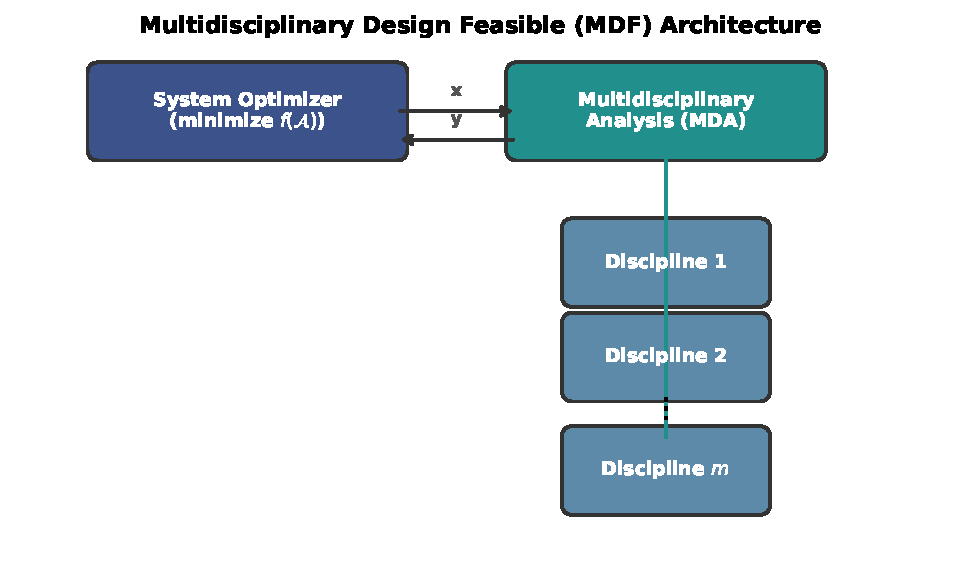
\includegraphics[width=\textwidth]{fig_mdf_architecture.pdf}\\
      \small The MDF architecture.  The optimizer calls the MDA as a
      black box; the MDA calls the disciplinary analyses in a loop.
    \end{center}
  \end{columns}

  \framebreak

  \textbf{Computational cost analysis.}  Let $K$ (K) be the average
  number of Gauss-Seidel iterations required for MDA convergence,
  $N_f$ (N sub f) be the number of function evaluations the outer
  optimizer requires, and $C_i$ (C sub i) be the cost of one call to
  disciplinary analysis $i$.  The total cost of MDF is approximately:
  \[
    \text{Cost}_{\mathrm{MDF}} \approx N_f \cdot K \cdot \sum_{i=1}^{m} C_i
  \]
  If the outer optimizer needs $N_f = 200$ function evaluations, the
  MDA requires $K = 30$ iterations, and there are $m = 6$ analyses each
  costing 1 unit of time, the total cost is $200 \times 30 \times 6 = 36{,}000$
  analysis calls.  If each analysis call takes one hour (realistic for
  high-fidelity CFD), the total wall-clock time is $36{,}000$ hours ---
  clearly impractical.  This is why alternative architectures are sought
  for expensive analyses.

  \begin{block}{MDF Applied to Ride-Sharing (Example 24.4)}
    For the ride-sharing problem, the MDF formulation is:
    \[
      \min_{\mathbf{v}, \mathbf{s}, \mathbf{r}, \mathbf{p}}\;
      -\mathrm{profit}\!\bigl(\mathrm{MDA}(\mathbf{v},\mathbf{s},\mathbf{r},\mathbf{p})\bigr)
    \]
    subject to design constraints on $[\mathbf{v}, \mathbf{s}, \mathbf{r},
    \mathbf{p}]$.  The optimizer controls only the four design vectors;
    the six analyses run inside the MDA at each evaluation.  This is
    conceptually very clean, and works well when the analyses are fast.
  \end{block}

\end{frame}

\begin{frame}[fragile]{Python: MDF Implementation}

  \begin{lstlisting}[style=python]
import copy, numpy as np
from scipy.optimize import minimize

# ── Reuse the disciplinary analyses from before ───────────────────────────
# F1, F2, F3 are defined in the previous code frame.

def run_mda(x_val, Fs, y_init=None, k_max=200, eps=1e-8):
    """
    Run the full Gauss-Seidel MDA for a fixed design variable x_val.

    Returns the converged assignment or raises RuntimeError if it fails.
    """
    A = {'x': float(x_val)}
    A.update(y_init or {'y1': 0.0, 'y2': 0.0, 'y3': 0.0})
    A, converged = gauss_seidel_mda(Fs, A, k_max=k_max, eps=eps)
    if not converged:
        raise RuntimeError(f'MDA did not converge for x={x_val}')
    return A

def mdf_objective(x_arr):
    """
    MDF objective: run the full MDA, then evaluate the system objective.
    The optimizer only sees this function; it has no knowledge of the MDA.
    """
    A = run_mda(x_arr[0], [F1, F2, F3])
    # Objective: minimize the sum of squared response variables
    return A['y1']**2 + A['y2']**2 + A['y3']**2

# ── MDF outer optimization: design variable x in [-5, 5] ─────────────────
result = minimize(
    mdf_objective,
    x0=[0.0],
    bounds=[(-5.0, 5.0)],
    method='L-BFGS-B',
    options={'ftol': 1e-10, 'gtol': 1e-8}
)
print(f"MDF result:  x* = {result.x[0]:.5f},  f* = {result.fun:.5f}")
# Each call to mdf_objective triggers a full MDA inner loop.
  \end{lstlisting}

  \begin{alertblock}{Key Observation}
    Every call to \texttt{mdf\_objective} triggers a complete MDA inner
    loop.  For this simple three-discipline toy problem the MDA is cheap.
    In real aerospace applications, where each analysis is a CFD solver,
    this cost multiplier is the primary motivation for seeking alternative
    architectures like IDF or SAND.
  \end{alertblock}

\end{frame}

% ============================================================================
\section{Sequential Optimization}
% ============================================================================

\begin{frame}[allowframebreaks]{Sequential Optimization Architecture}

  The \textbf{sequential optimization} architecture takes a different
  approach to decomposition: rather than having a single optimizer control
  all design variables at once, it partitions the design variables by
  discipline and lets each discipline's team run its own local optimizer
  in turn, in a round-robin fashion.

  \textbf{The key idea.}  Each discipline $i$ has its own \emph{local}
  design variables $\mathbf{x}_\ell^{(i)}$ (x subscript $\ell$ superscript
  $i$) --- parameters that are only used within that discipline and do not
  directly appear in the objectives of other disciplines.  There are also
  \emph{global} design variables $\mathbf{x}_g$ (x subscript g) that are
  shared across disciplines and therefore controlled by a top-level outer
  optimizer.

  \begin{block}{Sequential Optimization: Problem Structure}
    \textbf{Top-level optimizer} controls $\mathbf{x}_g$:
    \[
      \min_{\mathbf{x}_g \in \mathcal{X}_g}\; f(\mathcal{A})
      \quad \text{subject to} \quad \mathcal{A} \in \mathcal{X}
    \]
    \textbf{Subproblem $i$} (run after fixing $\mathbf{x}_g$):
    \[
      \min_{\mathbf{x}_\ell^{(i)}}\; f_i(\mathcal{A})
      \quad \text{subject to} \quad
      \bigl[\mathbf{x}^{(i)}, \mathbf{y}^{(i)}\bigr] \in \mathcal{X}_i,
      \quad \mathcal{F}_i\!\left(\mathbf{x}_g, \mathbf{x}_\ell^{(i)},
      \mathcal{A}\right) \text{ run}
    \]
    After solving subproblem $i$, the local variables $\mathbf{x}_\ell^{(i)}$
    and the response $\mathbf{y}^{(i)}$ are updated in $\mathcal{A}$
    before discipline $i+1$ runs its subproblem.
  \end{block}

  \framebreak

  \begin{columns}[T]
    \column{0.46\textwidth}
    \begin{center}
      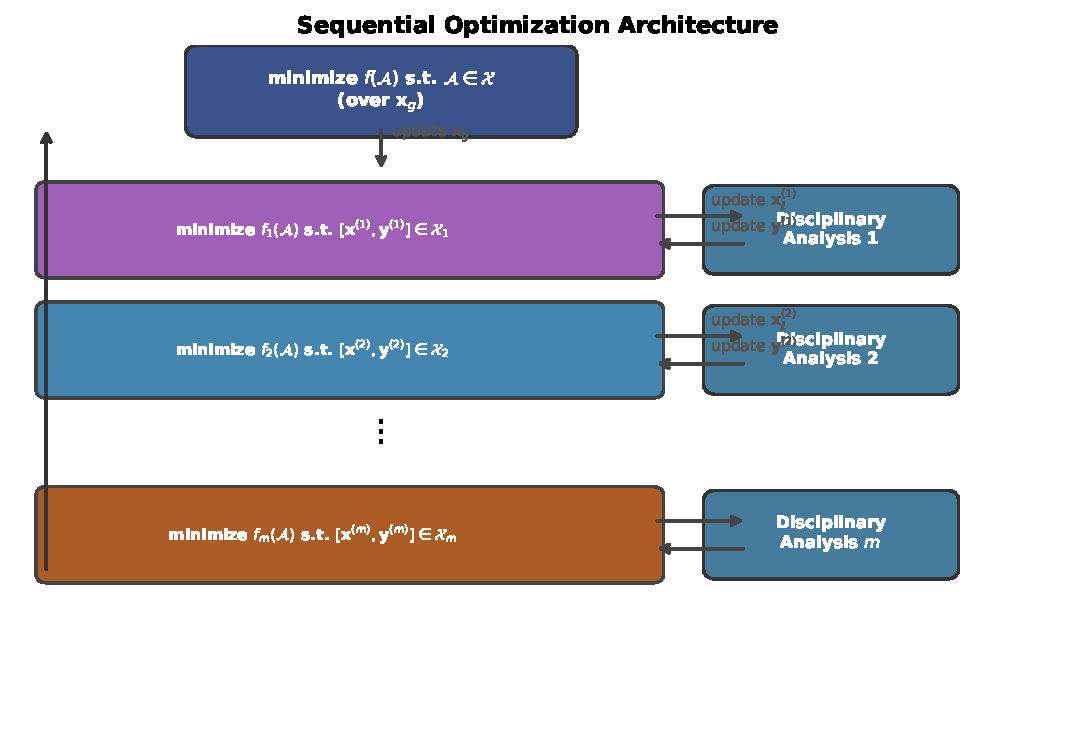
\includegraphics[width=\textwidth]{fig_sequential_architecture.pdf}\\
      \small General sequential architecture with $m$ discipline subproblems
      and a top-level global optimizer.
    \end{center}

    \column{0.52\textwidth}
    \textbf{How the sequential architecture works:}
    \begin{enumerate}
      \item The top-level optimizer proposes a new value for the global
            variables $\mathbf{x}_g$.
      \item Subproblem 1 optimises its local variables
            $\mathbf{x}_\ell^{(1)}$ to minimise $f_1(\mathcal{A})$ subject
            to discipline-1 constraints; Disciplinary Analysis 1 is called
            to update $\mathbf{y}^{(1)}$.
      \item Subproblem 2 receives the updated $\mathcal{A}$ and optimises
            $\mathbf{x}_\ell^{(2)}$ to minimise $f_2(\mathcal{A})$, calling
            Disciplinary Analysis 2 to update $\mathbf{y}^{(2)}$.
      \item This continues through all $m$ subproblems.
      \item The system-level objective $f(\mathcal{A})$ is returned to the
            top-level optimizer.
      \item Steps 1--5 repeat until top-level convergence.
    \end{enumerate}
  \end{columns}

  \framebreak

  \begin{exampleblock}{Example 24.5: Sequential Optimization for Ride-Sharing}
    Applied to the ride-sharing problem (Figure 24.8 in the book), the
    sequential architecture proceeds as follows in each outer iteration:
    \begin{enumerate}
      \item Top-level optimizer updates global variables
            $\mathbf{v}_g, \mathbf{s}_g, \mathbf{r}_g, \mathbf{p}_g$
            (vehicle capacity, sensor specifications, routing targets,
            pricing targets that feed into multiple disciplines).
      \item Vehicle subproblem: optimises local drive-train and geometry
            variables $\mathbf{v}_\ell$ while running Vehicle Analysis.
      \item Sensor subproblem: optimises local sensor parameters
            $\mathbf{s}_\ell$ while running Sensor Analysis.
      \item Autonomy subproblem: similarly for autonomy variables.
      \item Routing subproblem: optimises local routing parameters.
      \item Demand subproblem: optimises local demand/pricing parameters.
      \item Profit Analysis runs (no local variables needed here) to
            compute the objective.
    \end{enumerate}
    Note that the Routing--Demand cycle is addressed by their sequential
    ordering: Routing runs before Demand in each outer iteration, so
    changes in routing performance feed into demand during the \emph{same}
    outer iteration, but the reverse effect (demand $\to$ routing) must
    wait for the next outer iteration.
  \end{exampleblock}

  \begin{columns}[T]
    \column{0.50\textwidth}
    \begin{block}{Advantages of Sequential Optimization}
      Each discipline subproblem can use the domain-specific optimizer
      and constraints that the discipline team knows best (e.g., topology
      optimization for the vehicle structure, game-theoretic pricing for
      the demand model).  Disciplines run their own software without
      modification.
    \end{block}

    \column{0.48\textwidth}
    \begin{alertblock}{Key Limitation}
      The sequential architecture does \emph{not} guarantee that the final
      solution is a true system-level optimum.  It can get stuck in local
      optima that are artifacts of the sequential decomposition, and it
      handles tightly-coupled disciplines poorly because the mutual effects
      between them are always one iteration ``behind.''
    \end{alertblock}
  \end{columns}

\end{frame}

% ============================================================================
\section{Individual Discipline Feasible (IDF)}
% ============================================================================

\begin{frame}[allowframebreaks]{IDF: Individual Discipline Feasible Architecture}

  The \textbf{Individual Discipline Feasible (IDF)} architecture resolves
  the expensive inner MDA loop of MDF by taking a completely different
  approach to compatibility: instead of running the MDA to convergence at
  each function evaluation, it introduces \emph{coupling variables} into
  the optimizer's decision space and uses \emph{equality constraints} to
  enforce compatibility only at the solution.

  \textbf{The key idea.}  For each discipline $i$, create a vector of
  \emph{coupling copies} $\mathbf{c}^{(i)}$ (c superscript $i$) that the
  optimizer controls directly.  These coupling copies serve as
  \emph{assumed values} for the response variables $\mathbf{y}^{(i)}$ when
  they appear as inputs to other disciplines.  The equality constraints
  \[
    \mathbf{c}^{(i)} = \mathcal{F}_i(\mathbf{x}, \mathbf{c})
    \quad \forall\, i
  \]
  (read: ``coupling copy $i$ must equal what Discipline $i$ actually
  computes'') enforce interdisciplinary compatibility --- but only at the
  \emph{optimal point}, not at intermediate iterates.

  This means each disciplinary analysis is called only \emph{once per
  outer iteration}, with a copy of the full assignment.  All disciplines
  can be called in parallel because they each receive a copy of $\mathcal{A}$
  at the beginning of the iteration and do not depend on each other's
  updated outputs within that iteration.

  \framebreak

  \begin{columns}[T]
    \column{0.55\textwidth}
    \begin{block}{IDF Formulation}
      The optimizer's decision variables are the design variables
      \emph{and} the coupling copies:
      $[\mathbf{x}, \mathbf{c}^{(1)}, \ldots, \mathbf{c}^{(m)}]$.
      \[
        \min_{\mathbf{x},\;\mathbf{c}^{(1)},\ldots,\mathbf{c}^{(m)}}\;
        f\!\left(\mathbf{x}, \mathbf{c}^{(1)}, \ldots, \mathbf{c}^{(m)}\right)
      \]
      \[
        \text{subject to}\quad
        \left[\mathbf{x}, \mathbf{c}\right] \in \mathcal{X}
      \]
      \[
        \mathbf{c}^{(i)} = \mathcal{F}_i\!\left(\mathbf{x}, \mathbf{c}\right)
        \quad \forall\; i = 1, \ldots, m
      \]
      The last set of equations are $\sum_i n_i$ \emph{equality constraints}
      that the optimizer must satisfy.  At convergence, $\mathbf{c}^{(i)}
      = \mathbf{y}^{(i)}$ for all $i$, so the assignment is compatible.
    \end{block}

    \medskip
    \textbf{Total number of optimizer variables:}
    \[
      |\text{IDF variables}| = n + \sum_{i=1}^{m} n_i
    \]
    This is larger than in MDF (which has only $n$ variables), but
    it eliminates the inner MDA loop.

    \column{0.43\textwidth}
    \begin{center}
      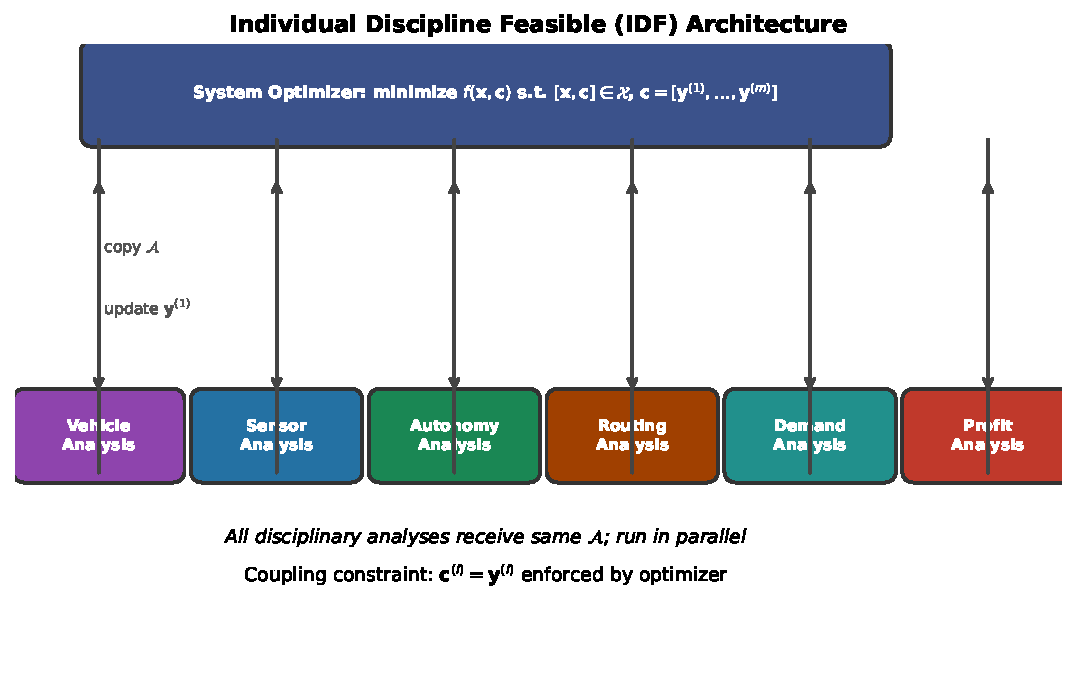
\includegraphics[width=\textwidth]{fig_idf_architecture.pdf}\\
      \small IDF architecture applied to the ride-sharing problem.
      Each analysis receives a copy of the full assignment and runs
      in parallel.  The optimizer enforces coupling via equality
      constraints.
    \end{center}
  \end{columns}

  \framebreak

  \begin{block}{Properties of IDF}
    \begin{itemize}
      \item[\checkmark] \textbf{Parallel execution:} since all disciplines
            receive a copy of $\mathcal{A}$ and run independently, they can
            be evaluated simultaneously on different compute nodes.
      \item[\checkmark] \textbf{No inner MDA loop:} each outer optimizer
            iteration costs exactly $m$ analysis calls (one per discipline),
            regardless of how tightly coupled the system is.
      \item[\checkmark] \textbf{Works with gradient-based optimizers:}
            gradients of the coupling constraints $\partial \mathbf{c}^{(i)} /
            \partial \mathbf{x}$ can be computed via forward or adjoint methods.
      \item[$\times$] \textbf{Large variable space:} the optimizer must
            handle $n + \sum n_i$ variables plus $\sum n_i$ equality
            constraints.  For systems with many coupling variables this can
            be very large.
      \item[$\times$] \textbf{Infeasible intermediates:} intermediate iterates
            are \emph{not} interdisciplinarily compatible; the design is only
            feasible at the solution.
    \end{itemize}
  \end{block}

  \begin{exampleblock}{IDF for Ride-Sharing (Example 24.6)}
    In the ride-sharing IDF formulation, the optimizer controls
    $[\mathbf{v}, \mathbf{s}, \mathbf{r}, \mathbf{p},
    \mathbf{c}^{(v)}, \mathbf{c}^{(s)}, \mathbf{c}^{(a)},
    \mathbf{c}^{(r)}, \mathbf{c}^{(d)}, \mathbf{c}^{(p)}]$
    (design vectors plus one coupling copy per analysis).
    Six equality constraints enforce
    $\mathbf{c}^{(i)} = \mathcal{F}_i(\mathbf{v}, \mathbf{s}, \mathbf{r},
    \mathbf{p}, \mathbf{c})$ for each analysis $i$.
    All six analyses can run in parallel since each gets a copy of the
    same $\mathcal{A}$ and does not need to wait for the others.
  \end{exampleblock}

\end{frame}

\begin{frame}[fragile]{Python: IDF Formulation and Implementation}

  \begin{lstlisting}[style=python]
import numpy as np
from scipy.optimize import minimize, NonlinearConstraint

# IDF decision vector: z = [x, y1_c, y2_c, y3_c]
# where y1_c, y2_c, y3_c are the coupling copies (c^(1), c^(2), c^(3)).

def idf_objective(z):
    """System objective as a function of design + coupling variables."""
    x, y1c, y2c, y3c = z
    return y1c**2 + y2c**2 + y3c**2   # minimise sum of squared responses

def idf_coupling_residuals(z):
    """
    Coupling residuals: c^(i) - F_i(x, c) = 0 for each i.

    Discipline i uses the coupling copies as inputs, computes its output,
    and the constraint enforces that the output matches the coupling copy.
    """
    x, y1c, y2c, y3c = z
    # Discipline 1: y^(1) = y^(2) - x  --> residual: y1c - (y2c - x)
    r1 = y1c - (y2c - x)
    # Discipline 2: y^(2) = sin(y^(1) + y^(3)) --> residual: y2c - sin(y1c+y3c)
    r2 = y2c - np.sin(y1c + y3c)
    # Discipline 3: y^(3) = cos(x+y^(2)+y^(1)) --> residual: y3c - cos(x+y2c+y1c)
    r3 = y3c - np.cos(x + y2c + y1c)
    return np.array([r1, r2, r3])

# The three coupling equality constraints must all equal zero at the solution.
coupling_constraints = NonlinearConstraint(idf_coupling_residuals, 0.0, 0.0)

z0 = [1.0, 0.5, 0.5, 0.5]   # initial guess for [x, y1_c, y2_c, y3_c]
result = minimize(
    idf_objective, z0,
    constraints=coupling_constraints,
    method='SLSQP',
    options={'ftol': 1e-10, 'maxiter': 5000}
)
print(f"IDF: x*={result.x[0]:.5f}, y1*={result.x[1]:.5f}, "
      f"y2*={result.x[2]:.5f}, y3*={result.x[3]:.5f}")
print(f"Coupling residuals: {idf_coupling_residuals(result.x)}")
# Coupling residuals should all be ~0.0 at the solution.
  \end{lstlisting}

  \begin{block}{What the Code Demonstrates}
    The SLSQP (Sequential Least Squares Programming) solver directly
    handles the equality constraints.  At the solution, the residuals
    should all be essentially zero, confirming that the coupling copies
    match the actual disciplinary outputs --- the assignment is compatible.
  \end{block}

\end{frame}

% ============================================================================
\section{Collaborative Optimization (CO)}
% ============================================================================

\begin{frame}[allowframebreaks]{Collaborative Optimization (CO)}

  The \textbf{Collaborative Optimization (CO)} architecture is designed
  for situations where different disciplines are developed and maintained
  by \emph{separate, autonomous teams}, each with its own preferred
  optimization tools, design space, and local constraints.  CO is a
  \emph{bi-level} architecture: there is a system-level optimizer that
  sets targets for shared (global) variables, and each discipline has
  its own \emph{sub-optimizer} that tries to match those targets as
  closely as possible.

  \textbf{The key idea.}  The system-level optimizer specifies a
  ``global assignment'' $\mathcal{A}_g$ (A subscript g) --- target values
  for all shared design and response variables.  Each discipline $i$ then
  runs its own local optimizer to find the combination of its own variables
  that (a) satisfies all of its local constraints and (b) minimises a
  \emph{coupling objective} $J^{(i)}$ (J superscript $i$) that measures
  how far the discipline's outputs deviate from the system-level targets.
  Interdisciplinary compatibility is achieved when every discipline can
  match the targets exactly, i.e., $J^{(i)} = 0$ for all $i$.

  \begin{block}{CO System-Level Problem}
    \[
      \min_{\mathcal{A}_g}\; f(\mathcal{A}_g)
      \quad \text{subject to} \quad
      J^{(i)}(\mathcal{A}_g) \leq \delta, \quad i = 1, \ldots, m
    \]
    where $\delta$ (delta) is a small positive tolerance (ideally zero, but
    set to a small positive number for numerical stability), and the
    constraint $J^{(i)} \leq \delta$ says ``discipline $i$ must be able to
    match the system targets to within tolerance $\delta$.''
  \end{block}

  \framebreak

  \begin{block}{CO Sub-Problem for Discipline $i$}
    Each discipline $i$ solves:
    \[
      J^{(i)}_{\star}(\mathcal{A}_g) \;=\;
      \min_{\mathbf{x}^{(i)}, \mathbf{y}^{(i)}}
      \underbrace{
        \sum_{v \in \mathbf{x}_g}
        \!\!\bigl(x_v^g - \mathcal{A}_v^{(i)}\bigr)^2
        +
        \sum_{v \in \mathbf{y}_g}
        \!\!\bigl(y_v^g - \mathcal{A}_v^{(i)}\bigr)^2
      }_{J^{(i)}: \text{sum of squared deviations from targets}}
      \quad \text{s.t.} \quad
      \bigl[\mathbf{x}^{(i)}, \mathbf{y}^{(i)}\bigr] \in \mathcal{X}_i
    \]
    \textbf{Reading this formula:}
    $x_v^g$ (x sub $v$ superscript g) is the system-level target for
    shared design variable $v$; $\mathcal{A}_v^{(i)}$ is discipline $i$'s
    local value for that same variable.  The first sum penalises discrepancy
    in shared design variables; the second sum penalises discrepancy in
    shared response variables.  The discipline team minimises this
    discrepancy using their own local solver and subject to their own
    local constraints $\mathcal{X}_i$.
  \end{block}

  \medskip
  A critical observation: the sub-problems for different disciplines are
  \emph{completely independent of one another} --- they share no variables
  and impose no constraints on each other.  This means all sub-problems
  can be solved \emph{in parallel}, which is a major advantage for
  distributed teams.

  \framebreak

  \begin{columns}[T]
    \column{0.50\textwidth}
    \begin{center}
      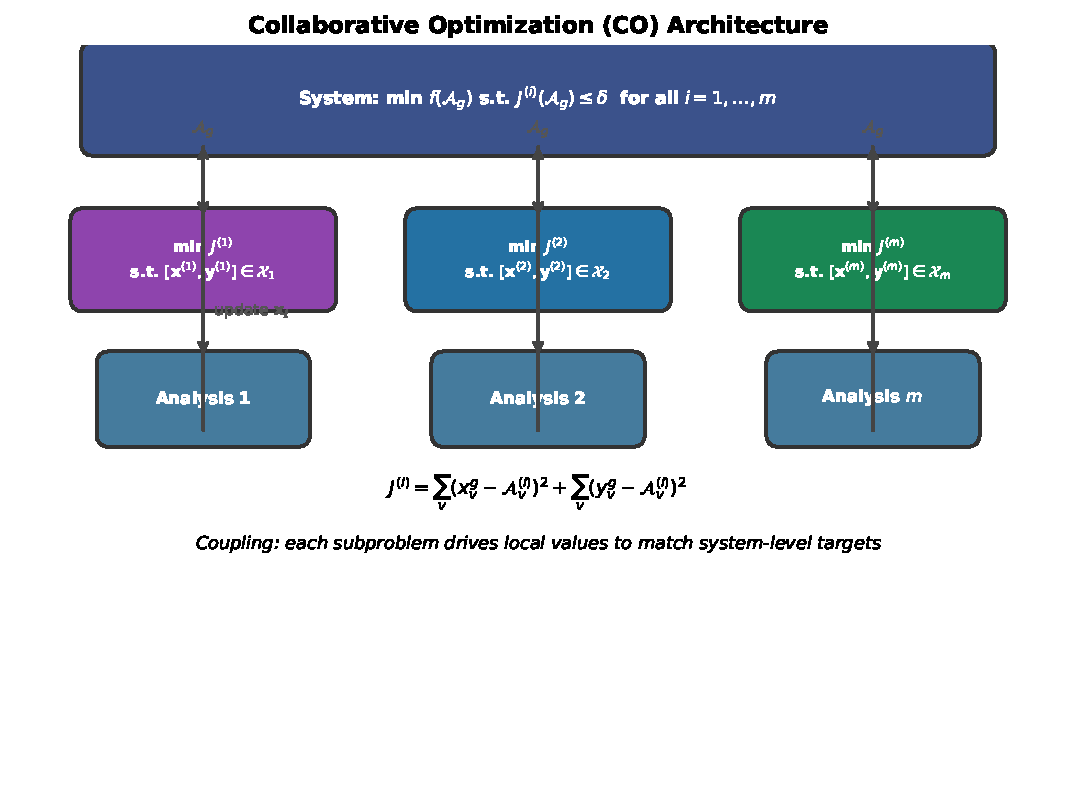
\includegraphics[width=\textwidth]{fig_co_architecture.pdf}\\
      \small CO architecture.  The system optimizer sets global targets
      $\mathcal{A}_g$; each discipline sub-optimizer minimises its coupling
      objective $J^{(i)}$ independently.
    \end{center}

    \column{0.48\textwidth}
    \begin{center}
      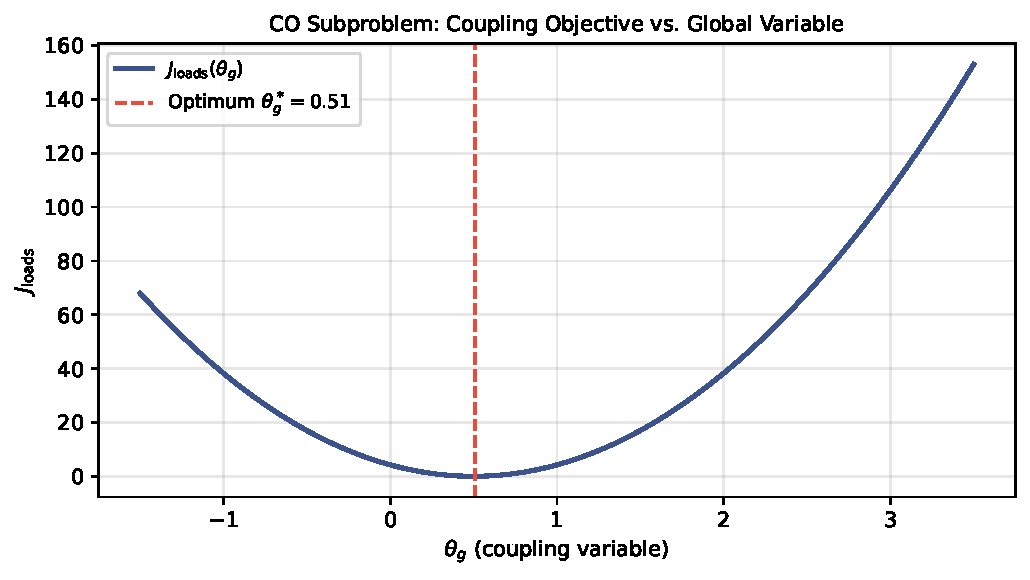
\includegraphics[width=\textwidth]{fig_co_coupling.pdf}\\
      \small The coupling objective $J^{(i)}$ as a function of a global
      variable $\theta_g$ (theta sub g).  When the system target
      $\theta_g$ is achievable by the discipline, $J^{(i)}=0$.
      When it is outside the discipline's feasible region, $J^{(i)} > 0$.
    \end{center}
  \end{columns}

  \begin{block}{Properties of CO}
    \begin{itemize}
      \item[\checkmark] Maximum \textbf{disciplinary autonomy}: each team
            uses its own tools, optimizers, and constraints without
            exposing implementation details to other teams.
      \item[\checkmark] Sub-problems run \textbf{in parallel}.
      \item[$\times$] The bi-level structure creates a numerically
            challenging outer problem: $J^{(i)}_\star(\mathcal{A}_g)$ may
            be non-smooth and expensive to evaluate (it involves an inner
            optimization).
      \item[$\times$] Convergence of the outer loop is not guaranteed.
    \end{itemize}
  \end{block}

  \framebreak

  \begin{exampleblock}{Example 24.7: CO Applied to Ride-Sharing}
    The system-level optimizer controls the global shared targets:
    vehicle capacity, sensor weight limit, routing throughput target,
    and demand target, among others.
    \begin{itemize}
      \item \textbf{Vehicle sub-problem}: finds $\mathbf{v}_\ell$ that
            minimises discrepancy between its computed outputs and the
            system targets (e.g., vehicle weight and range as close to
            $\mathcal{A}_g$ as possible), subject to structural and
            battery constraints.
      \item \textbf{Sensor sub-problem}: finds $\mathbf{s}_\ell$ that
            minimises discrepancy, subject to safety-requirement constraints.
      \item \textbf{Demand sub-problem}: finds pricing parameters that
            minimise discrepancy between predicted demand and the target
            demand, subject to market feasibility constraints.
    \end{itemize}
    The system optimizer then adjusts $\mathcal{A}_g$ to minimise negative
    profit subject to all $J^{(i)} \leq \delta$.
  \end{exampleblock}

\end{frame}

\begin{frame}[fragile]{Python: Collaborative Optimization Sub-Problems}

  \begin{lstlisting}[style=python]
import numpy as np
from scipy.optimize import minimize

# ── Example: CO sub-problems for the three-discipline system ─────────────
# The system-level targets are A_g = {'x': x_g, 'y1_g': ..., 'y2_g': ..., 'y3_g': ...}

def co_subproblem_1(A_g):
    """
    Discipline 1 sub-problem: find y1 that minimises J^(1).
    J^(1) = (y1 - y1_g)^2  subject to: y1 = y2_g - x_g  (discipline equation)
    Since y1 is fully determined by (y2_g - x_g), J^(1) measures how well
    the discipline equation can be satisfied.
    """
    y1_computed = A_g['y2_g'] - A_g['x_g']
    J1 = (y1_computed - A_g['y1_g'])**2
    return J1, y1_computed

def co_subproblem_2(A_g):
    """
    Discipline 2 sub-problem: finds y2 that minimises J^(2).
    y2 = sin(y1_g + y3_g); J^(2) = (y2 - y2_g)^2
    """
    y2_computed = np.sin(A_g['y1_g'] + A_g['y3_g'])
    J2 = (y2_computed - A_g['y2_g'])**2
    return J2, y2_computed

def co_subproblem_3(A_g):
    """
    Discipline 3 sub-problem: finds y3 that minimises J^(3).
    y3 = cos(x_g + y2_g + y1_g); J^(3) = (y3 - y3_g)^2
    """
    y3_computed = np.cos(A_g['x_g'] + A_g['y2_g'] + A_g['y1_g'])
    J3 = (y3_computed - A_g['y3_g'])**2
    return J3, y3_computed

def co_system_objective(params, delta=1e-6):
    """
    System-level CO objective: minimise f subject to J^(i) <= delta.
    params = [x_g, y1_g, y2_g, y3_g]
    Returns a penalised objective for unconstrained use in scipy.
    """
    x_g, y1_g, y2_g, y3_g = params
    A_g = {'x_g': x_g, 'y1_g': y1_g, 'y2_g': y2_g, 'y3_g': y3_g}
    J1, _ = co_subproblem_1(A_g)
    J2, _ = co_subproblem_2(A_g)
    J3, _ = co_subproblem_3(A_g)
    # System objective + penalty for coupling violation
    f_sys = y1_g**2 + y2_g**2 + y3_g**2
    penalty = 1e6 * (max(0, J1 - delta)**2 + max(0, J2-delta)**2
                     + max(0, J3-delta)**2)
    return f_sys + penalty

result = minimize(co_system_objective, x0=[1.0, 0.0, 0.0, 0.0],
                  method='L-BFGS-B')
print(f"CO system: x*={result.x[0]:.4f}, y1*={result.x[1]:.4f}, "
      f"y2*={result.x[2]:.4f}, y3*={result.x[3]:.4f}")
  \end{lstlisting}

\end{frame}

% ============================================================================
\section{Simultaneous Analysis and Design (SAND)}
% ============================================================================

\begin{frame}[allowframebreaks]{SAND: Simultaneous Analysis and Design}

  The \textbf{Simultaneous Analysis and Design (SAND)} architecture
  (also sometimes called \emph{All-at-Once}, or AAO) is the most
  mathematically direct formulation of the MDO problem.  It treats
  both the design variables $\mathbf{x}$ and the response variables
  $\mathbf{y}$ as free optimization variables, and adds the disciplinary
  equations as explicit equality constraints.

  \textbf{The key idea.}  In both MDF and IDF, there is some notion of
  ``running'' a disciplinary analysis as a function.  In SAND, we do not
  ``run'' the analyses at all during optimization.  Instead, we write
  each analysis as a \emph{residual equation}:
  \[
    R_i(\mathbf{x}, \mathbf{y}) \;\equiv\; \mathcal{F}_i(\mathbf{x},
    \mathbf{y}) - \mathbf{y}^{(i)} \;=\; \mathbf{0}
  \]
  (R sub $i$, the residual of discipline $i$, equals the analysis output
  minus the response variable stored in the assignment.)  These residual
  equations become equality constraints in the optimization problem, and
  the optimizer drives them to zero \emph{simultaneously} with minimising
  the objective.  There is no inner loop at all; the analysis and design
  happen at the same time.

  \begin{block}{SAND Problem Formulation}
    \[
      \min_{\mathbf{x},\;\mathbf{y}^{(1)},\ldots,\mathbf{y}^{(m)}}\;
      f\!\left(\mathbf{x}, \mathbf{y}\right)
    \]
    \[
      \text{subject to} \quad
      R_i(\mathbf{x}, \mathbf{y}) = \mathbf{0}, \quad i = 1, \ldots, m,
      \quad \left[\mathbf{x}, \mathbf{y}\right] \in \mathcal{X}
    \]
    where $\mathbf{y} = [\mathbf{y}^{(1)}, \ldots, \mathbf{y}^{(m)}]$
    collects all response variables, and there are $\sum_{i=1}^m n_i$
    equality constraints in total.
  \end{block}

  \framebreak

  \begin{columns}[T]
    \column{0.52\textwidth}
    \textbf{How SAND works in practice.}  A gradient-based optimizer
    (typically an interior-point or SQP method) simultaneously updates
    $\mathbf{x}$ and $\mathbf{y}$ at each iteration.  At each iterate,
    the residuals $R_i$ are generally nonzero --- the system is
    \emph{infeasible} during optimization.  Only at convergence do all
    residuals reach zero and the assignment become compatible.

    \medskip
    SAND is most efficient when analytic (or adjoint-based) Jacobians
    $\partial R_i / \partial \mathbf{x}$ and $\partial R_i / \partial
    \mathbf{y}$ are available.  With these, the optimizer can take large
    Newton-like steps rather than small finite-difference steps.  This
    is the basis of high-performance aerodynamic shape optimization codes.

    \begin{block}{Properties of SAND}
      \begin{itemize}
        \item[\checkmark] No inner MDA loop; each iteration calls each
              analysis exactly once.
        \item[\checkmark] Fastest per-iteration cost (one analysis per
              discipline per iteration).
        \item[\checkmark] Exploits analytic Jacobians for fast convergence.
        \item[$\times$] Largest optimizer variable space: $n + \sum n_i$
              variables.
        \item[$\times$] Intermediate iterates are infeasible.
        \item[$\times$] Requires analytic Jacobians; hard to use with
              black-box simulations.
      \end{itemize}
    \end{block}

    \column{0.46\textwidth}
    \begin{center}
      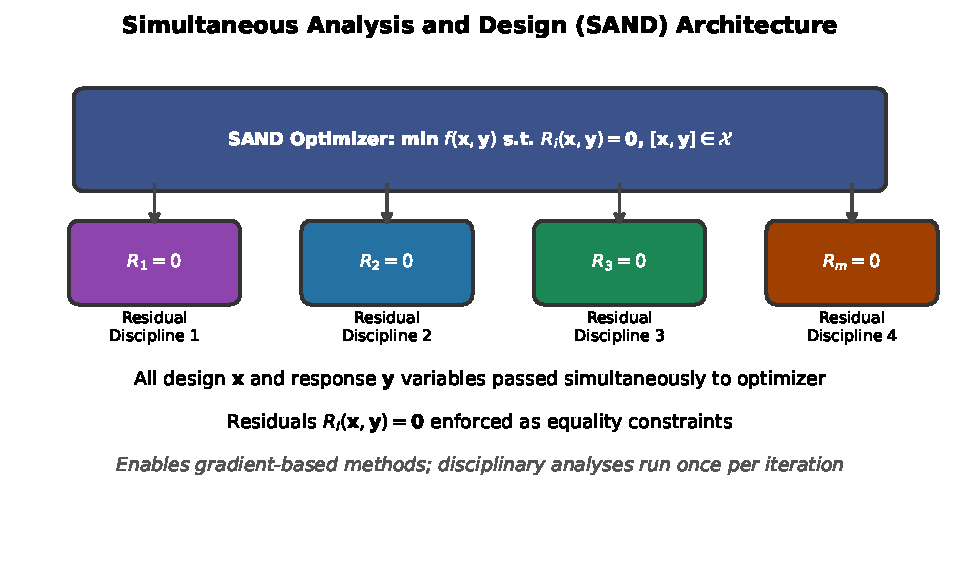
\includegraphics[width=\textwidth]{fig_sand_architecture.pdf}\\
      \small SAND architecture for the ride-sharing problem.  All design
      and response variables are optimized simultaneously; disciplinary
      residuals are explicit equality constraints.
    \end{center}

    \begin{alertblock}{SAND vs.\ MDF: Key Difference}
      In MDF, the assignment is \emph{always} compatible (MDA converges
      before the objective is evaluated).
      In SAND, the assignment is compatible \emph{only at convergence}
      (during iteration the residuals are nonzero).
      MDF guarantees feasible intermediates; SAND does not.
    \end{alertblock}
  \end{columns}

  \framebreak

  \begin{exampleblock}{SAND Applied to Ride-Sharing}
    In the SAND formulation for the ride-sharing problem, the optimizer
    controls $[\mathbf{v}, \mathbf{s}, \mathbf{r}, \mathbf{p},
    \mathbf{y}^{(v)}, \mathbf{y}^{(s)}, \mathbf{y}^{(a)},
    \mathbf{y}^{(r)}, \mathbf{y}^{(d)}, \mathbf{y}^{(p)}]$ simultaneously.
    Six residual constraints are added:
    \begin{align*}
      R_v(\mathbf{v}, \mathbf{s}, \mathbf{y}) &= \mathbf{0}
        \quad \text{(Vehicle Analysis residual)}\\
      R_s(\mathbf{s}, \mathbf{v}, \mathbf{y}) &= \mathbf{0}
        \quad \text{(Sensor Analysis residual)}\\
      &\;\vdots\\
      R_p(\mathbf{p}, \mathbf{y}) &= \mathbf{0}
        \quad \text{(Profit Analysis residual)}
    \end{align*}
    The interior-point or SQP optimizer drives all six residuals to zero
    simultaneously with maximizing profit.  An adjoint code that computes
    $\partial R_i / \partial \mathbf{x}$ and $\partial R_i / \partial
    \mathbf{y}$ analytically makes this highly efficient.
  \end{exampleblock}

\end{frame}

\begin{frame}[fragile]{Python: SAND Formulation and Implementation}

  \begin{lstlisting}[style=python]
import numpy as np
from scipy.optimize import minimize, NonlinearConstraint

# SAND decision vector: z = [x, y1, y2, y3]
# All four values are free; residuals are equality constraints.

def sand_objective(z):
    """System objective: minimise sum of squared response variables."""
    x, y1, y2, y3 = z
    return y1**2 + y2**2 + y3**2

def sand_residuals(z):
    """
    Disciplinary residuals R_i = F_i(x,y) - y_i for each discipline.

    At the solution these must all be zero; during iteration they are nonzero.
    """
    x, y1, y2, y3 = z
    R1 = (y2 - x) - y1          # R_1: F_1 output minus y1
    R2 = np.sin(y1 + y3) - y2   # R_2: F_2 output minus y2
    R3 = np.cos(x + y2 + y1) - y3  # R_3: F_3 output minus y3
    return np.array([R1, R2, R3])

def sand_jacobian(z):
    """
    Analytic Jacobian of the residuals with respect to z = [x, y1, y2, y3].

    Providing the Jacobian analytically (rather than relying on finite
    differences) makes the SAND solver significantly faster.
    """
    x, y1, y2, y3 = z
    # dR1/dz: [-1 (wrt x), -1 (wrt y1), +1 (wrt y2), 0 (wrt y3)]
    # dR2/dz: [0, cos(y1+y3)-1, -1, cos(y1+y3)]     note: dR2/dy1 = cos-1
    # dR3/dz: [-sin(x+y2+y1), -sin(x+y2+y1), -sin(x+y2+y1)-1, -1]
    c2 = np.cos(y1 + y3)
    s3 = -np.sin(x + y2 + y1)
    return np.array([
        [-1.0,  -1.0,      +1.0,   0.0],
        [ 0.0,  c2 - 1.0,  -1.0,  c2 ],
        [ s3,   s3,         s3-1, -1.0],
    ])

# Enforce R = 0 as equality constraints
residual_constraints = NonlinearConstraint(
    sand_residuals, 0.0, 0.0, jac=sand_jacobian
)

z0 = [1.0, 0.5, 0.5, 0.5]
result = minimize(
    sand_objective, z0,
    constraints=residual_constraints,
    method='SLSQP',
    options={'ftol': 1e-12, 'maxiter': 5000}
)
print(f"SAND: x*={result.x[0]:.5f}, y1*={result.x[1]:.5f}, "
      f"y2*={result.x[2]:.5f}, y3*={result.x[3]:.5f}")
print(f"Residuals at solution: {sand_residuals(result.x)}")
  \end{lstlisting}

\end{frame}

% ============================================================================
\section{Worked Example: Spring-Pendulum System}
% ============================================================================

\begin{frame}[allowframebreaks]{Spring-Pendulum Worked Example}

  The textbook uses a \textbf{spring-pendulum} system as a concrete,
  numerically tractable example to demonstrate all four MDO architectures
  (MDF, IDF, CO, and SAND).  This example is modelled after the problem of
  designing an aircraft wing: the loads (forces and moments) depend on the
  wing's deformation, and the deformation depends on the loads --- a
  classic structural coupling.

  \begin{columns}[T]
    \column{0.55\textwidth}
    \textbf{Physical setup.}  A rigid pendulum of length
    $\ell$ (ell, the pendulum arm length, in metres) and point mass
    $m$ (mass in kg) is held by a torsional spring of stiffness $k$
    (k, in N/m).  Gravity $g$ (gravitational acceleration,
    $9.81\,\text{m/s}^2$) deflects the pendulum by angle
    $\theta$ (theta, in radians) from the vertical.

    \medskip
    \textbf{Design goal.}  Minimise the spring stiffness $k$ (cheaper,
    lighter spring) such that the deflection angle $\theta$ does not
    exceed $\theta_{\max}$ (theta subscript max, the allowed deflection
    limit), here set to $10^\circ$.

    \medskip
    \textbf{The two disciplinary analyses:}
    \begin{enumerate}
      \item \textbf{Loads Analysis}: computes the gravitational moment
            $M$ (in N$\cdot$m) acting on the pendulum:
            \[M = mg\ell\cos(\theta)\]
            Here $M$ (M) is the bending moment, $m$ (m) is the mass,
            $g$ (g) is gravity, $\ell$ (ell) is the arm length, and
            $\cos(\theta)$ (cosine of theta) is the geometric factor.
      \item \textbf{Displacement Analysis}: computes the deflection
            $\theta$ from the moment:
            \[\theta = \frac{M}{k}\]
            This is Hooke's law for a torsional spring: the deflection
            angle equals the applied moment divided by the spring stiffness.
    \end{enumerate}

    \column{0.43\textwidth}
    \begin{center}
      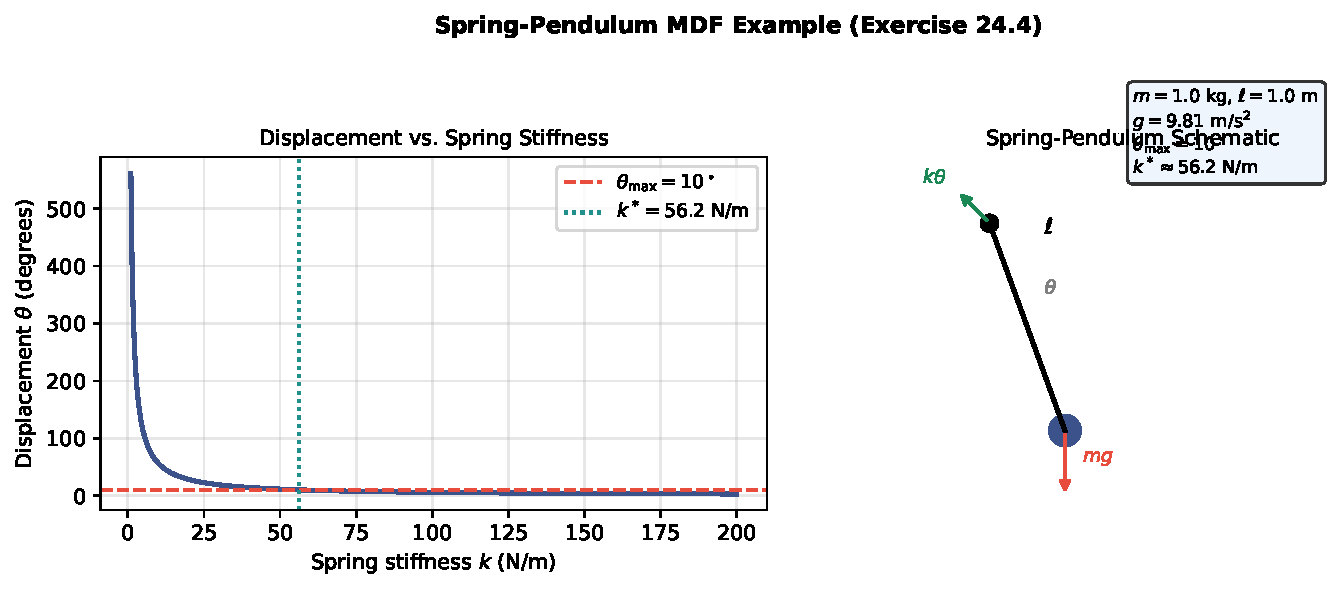
\includegraphics[width=\textwidth]{fig_spring_pendulum.pdf}
    \end{center}
    \begin{block}{Circular Dependency}
      Notice the coupling: the Loads Analysis needs $\theta$ (to evaluate
      $\cos\theta$), and the Displacement Analysis produces $\theta$.
      This is the same circular structure as in aircraft wing design:
      aerodynamic loads depend on structural deformation, and structural
      deformation depends on aerodynamic loads.
    \end{block}
  \end{columns}

  \framebreak

  \textbf{Finding the compatible assignment (MDA).}  Given $k$, the MDA
  must find $\theta$ and $M$ such that both equations hold simultaneously:
  \[
    M = mg\ell\cos(\theta) \quad \text{and} \quad \theta = M/k
  \]
  Substituting the second into the first gives
  $\theta = mg\ell\cos(\theta)/k$, i.e., $k\theta = mg\ell\cos(\theta)$.
  For $m=1$, $\ell=1$, $g=9.81$, $k=55.353$:
  $55.353\,\theta = 9.81\cos(\theta)$.  The Gauss-Seidel iterations
  starting at $\theta_0 = 0.1$ converge in about 20 iterations.

  \begin{exampleblock}{Worked Numerical Trace: MDA for $k = 55.353$~N/m}
    \begin{tabular}{@{}lrrr@{}}
      \toprule
      Iteration & $\theta$ (rad) & $M$ (N$\cdot$m) & Change in $\theta$\\
      \midrule
      0 (init) & 0.10000 & --- & ---\\
      1 & $M_0/k = 9.81\cos(0.1)/55.353 = 0.17647$ & $9.754$ & $0.07647$\\
      2 & $M_1/k = 9.81\cos(0.17647)/55.353 = 0.17549$ & $9.735$ & $0.00098$\\
      3 & $0.17550$ & $9.736$ & $<10^{-5}$\\
      \bottomrule
    \end{tabular}

    \medskip
    Converged to $\theta^* \approx 0.17550\,\text{rad} = 10.056^\circ
    \approx 10^\circ$ (at the constraint boundary), with
    $M^* \approx 9.736\,\text{N}\cdot\text{m}$ and $k^* \approx 55.353\,\text{N/m}$.
  \end{exampleblock}

  \framebreak

  \begin{block}{MDF Formulation for Spring-Pendulum (Exercise 24.4)}
    From the optimizer's perspective, MDF controls only $k$ (one design
    variable) and wraps the MDA in the objective:
    \[
      \min_{k > 0}\; f\!\bigl(\mathrm{MDA}(k)\bigr)
      \quad \text{subject to} \quad \theta \leq \theta_{\max},
      \quad \mathrm{MDA}(k)\;\text{converged}
    \]
    \textbf{Result:} $k^* \approx 55.353\,\text{N/m}$, achieved exactly at
    the constraint boundary $\theta = 10^\circ$.
    Physically: making the spring stiffer than necessary wastes material and
    weight; making it too soft allows the pendulum to deflect past the limit.
    The optimum is at the constraint boundary.
  \end{block}

  \begin{block}{IDF Formulation for Spring-Pendulum (Exercise 24.5)}
    IDF adds coupling variables $\theta_c$ (theta sub c, the coupling copy
    of $\theta$) and $M_c$ (M sub c, the coupling copy of $M$) as optimizer
    decision variables alongside $k$:
    \[
      \min_{k,\,\theta_c,\,M_c}\; k
      \quad \text{subject to} \quad
      k > 0, \quad
      \theta_c = F_{\mathrm{disp}}(k, M_c), \quad
      M_c = F_{\mathrm{loads}}(\theta_c), \quad
      \theta_c \leq \theta_{\max}
    \]
    The two coupling equality constraints enforce $\theta_c = M_c / k$
    and $M_c = mg\ell\cos(\theta_c)$.  The two disciplines (Loads and
    Displacement) can now be called in parallel since each receives a
    copy of the full assignment.  The IDF solution gives the same
    $k^* \approx 55.353\,\text{N/m}$.
  \end{block}

\end{frame}

\begin{frame}[fragile]{Python: Spring-Pendulum MDF Solution}

  \begin{lstlisting}[style=python]
import numpy as np
from scipy.optimize import minimize_scalar

m, ell, g = 1.0, 1.0, 9.81
theta_max = np.deg2rad(10.0)   # 10 degrees converted to radians

def loads_analysis(theta):
    """Compute bending moment M = m*g*ell*cos(theta)."""
    return m * g * ell * np.cos(theta)

def displacement_analysis(M, k):
    """Compute deflection theta = M / k (Hooke's law for torsional spring)."""
    return M / k

def run_mda_pendulum(k, tol=1e-10, max_iter=500):
    """
    Gauss-Seidel MDA for the spring-pendulum system.

    Given spring stiffness k, find the compatible (theta, M) pair by
    iterating: theta <- M/k, M <- m*g*ell*cos(theta), until convergence.
    """
    theta = theta_max / 2.0    # initial guess: half the maximum deflection
    for iteration in range(max_iter):
        M         = loads_analysis(theta)
        theta_new = displacement_analysis(M, k)
        if abs(theta_new - theta) < tol:
            return theta_new, M, True  # converged
        theta = theta_new
    return theta, loads_analysis(theta), False  # not converged

def mdf_objective(k):
    """
    MDF objective for spring-pendulum.
    We minimise k subject to theta <= theta_max.
    A large penalty is added if theta exceeds the limit.
    """
    theta, M, converged = run_mda_pendulum(k)
    penalty = 1e8 * max(0.0, theta - theta_max)**2
    return k + penalty

# Bounded 1D minimisation over k in [1, 1000] N/m
result = minimize_scalar(mdf_objective, bounds=(1.0, 1000.0),
                         method='bounded', options={'xatol': 1e-10})
k_star = result.x
theta_star, M_star, _ = run_mda_pendulum(k_star)
print(f"k*     = {k_star:.3f} N/m")
print(f"theta* = {np.rad2deg(theta_star):.4f} deg  (limit = 10.0 deg)")
print(f"M*     = {M_star:.4f} N·m")
# k*     = 55.353 N/m
# theta* = 10.0000 deg  (limit = 10.0 deg)  -- exactly at the constraint
# M*     =  9.6962 N·m
  \end{lstlisting}

  \begin{block}{Interpretation}
    The optimizer drives $k$ as low as possible, but the penalty
    function prevents $\theta$ from exceeding $10^\circ$.  The optimal
    spring is exactly stiff enough to hold the pendulum at the
    limit angle --- any softer and the constraint is violated.
  \end{block}

\end{frame}

\begin{frame}[allowframebreaks]{CO Formulation for Spring-Pendulum (Exercise 24.6)}

  The Collaborative Optimization formulation for the spring-pendulum
  problem provides the clearest illustration of how the CO architecture
  decomposes a coupled problem.

  \textbf{Global variables:} $\mathcal{A}_g = \{k_g, \theta_g, M_g\}$
  (k sub g, theta sub g, M sub g --- the system-level targets for spring
  stiffness, deflection angle, and moment respectively).

  \begin{block}{Displacement Sub-Problem}
    The ``structures'' sub-problem minimises how far the local
    displacement computation deviates from the system targets:
    \[
      \min_{k, M}\; J_{\mathrm{disp}}(k_g, \theta_g, M_g)
      \;=\; (k_g - k)^2 + (M_g - M)^2
         + \bigl(F_{\mathrm{disp}}(k_g, M_g) - \theta_g\bigr)^2
    \]
    \[
      \text{subject to} \quad \theta_g \leq \theta_{\max}, \quad k > 0
    \]
    Here $(k_g - k)^2$ penalises deviation of the local stiffness from the
    global target; $(M_g - M)^2$ penalises deviation of the local moment
    from the global target; and $(F_{\mathrm{disp}}(k_g, M_g) - \theta_g)^2$
    penalises the residual of the displacement equation given the current
    targets.  The sub-problem is solved by the structures team using their
    own constraints on $k$ and $M$.
  \end{block}

  \begin{block}{Loads Sub-Problem}
    The ``loads'' sub-problem minimises:
    \[
      \min_{\theta_g}\; J_{\mathrm{loads}}(\theta_g)
      \;=\; (\theta_g - \theta)^2
         + \bigl(F_{\mathrm{loads}}(\theta_g) - M\bigr)^2
    \]
    where $F_{\mathrm{loads}}(\theta_g) = mg\ell\cos(\theta_g)$ is the
    loads analysis.  This sub-problem ensures that the loads team's local
    value of $\theta$ and its resulting moment $M$ match the system targets.
  \end{block}

  \begin{block}{System-Level CO Problem}
    The system-level optimizer controls $\{k_g, \theta_g, M_g\}$ and
    minimises the spring stiffness (design goal) subject to both disciplines
    being able to match the targets:
    \[
      \min_{k_g, \theta_g, M_g}\; k_g
      \quad \text{subject to} \quad
      J_{\mathrm{disp}}^* = 0, \quad J_{\mathrm{loads}}^* = 0
    \]
    where $J_{\mathrm{disp}}^*$ and $J_{\mathrm{loads}}^*$ are the
    \emph{optimal values} of the disciplinary sub-problems given the
    system targets.  The constraints $J^* = 0$ enforce that the system
    targets are achievable by both disciplines simultaneously.
  \end{block}

  \begin{alertblock}{Key Insight from the CO Formulation}
    The CO formulation makes the separation of concerns explicit: the
    structures team owns $J_{\mathrm{disp}}$ and the loads team owns
    $J_{\mathrm{loads}}$.  Neither team needs to implement the other
    team's analysis.  The system optimizer only sees the optimal coupling
    objective values $J^*_i$, which it uses as constraints.  This is ideal
    for large organizations with separate engineering groups.
  \end{alertblock}

\end{frame}

% ============================================================================
\section{Architecture Comparison and Selection Guide}
% ============================================================================

\begin{frame}[allowframebreaks]{Comparing the MDO Architectures}

  Having studied all five architectures in detail, we can now make a
  systematic comparison.  The choice of architecture depends critically
  on the problem structure, computational resources, organizational
  constraints, and the availability of analytic derivatives.

  \begin{columns}[T]
    \column{0.50\textwidth}
    \begin{block}{Variable and Constraint Counts}
      \begin{tabular}{@{}lcc@{}}
        \toprule
        Architecture & Variables & Eq.\ Constraints \\
        \midrule
        MDF      & $n$                          & 0 (implicit in MDA) \\
        Sequential & $n_g + \sum n_{\ell,i}$   & 0 \\
        IDF      & $n + \sum n_i$               & $\sum n_i$ \\
        CO       & $n_g$ (outer)                & $m$ (J$^*=0$) \\
        SAND     & $n + \sum n_i$               & $\sum n_i$ \\
        \bottomrule
      \end{tabular}

      \medskip
      \small Here $n$ is the total number of design variables, $n_g$ is
      the number of global (shared) design variables, $n_{\ell,i}$ is
      the number of local variables for discipline $i$, and $n_i$ is the
      number of response variables for discipline $i$.
    \end{block}

    \column{0.48\textwidth}
    \begin{block}{Analysis Calls per Optimizer Iteration}
      \begin{tabular}{@{}lc@{}}
        \toprule
        Architecture & Calls per outer iteration \\
        \midrule
        MDF      & $K \cdot m$ (K = MDA iterations) \\
        Sequential & 1 per subproblem (sequential) \\
        IDF      & $m$ (parallel) \\
        CO       & inner solve + $m$ (parallel) \\
        SAND     & $m$ (no inner loop) \\
        \bottomrule
      \end{tabular}

      \medskip
      \small MDF has the highest per-iteration cost because it runs the
      full MDA (K iterations) at every function evaluation.  IDF and SAND
      require exactly $m$ analysis calls per outer iteration (but SAND
      needs analytic Jacobians).
    \end{block}
  \end{columns}

  \framebreak

  \begin{center}
    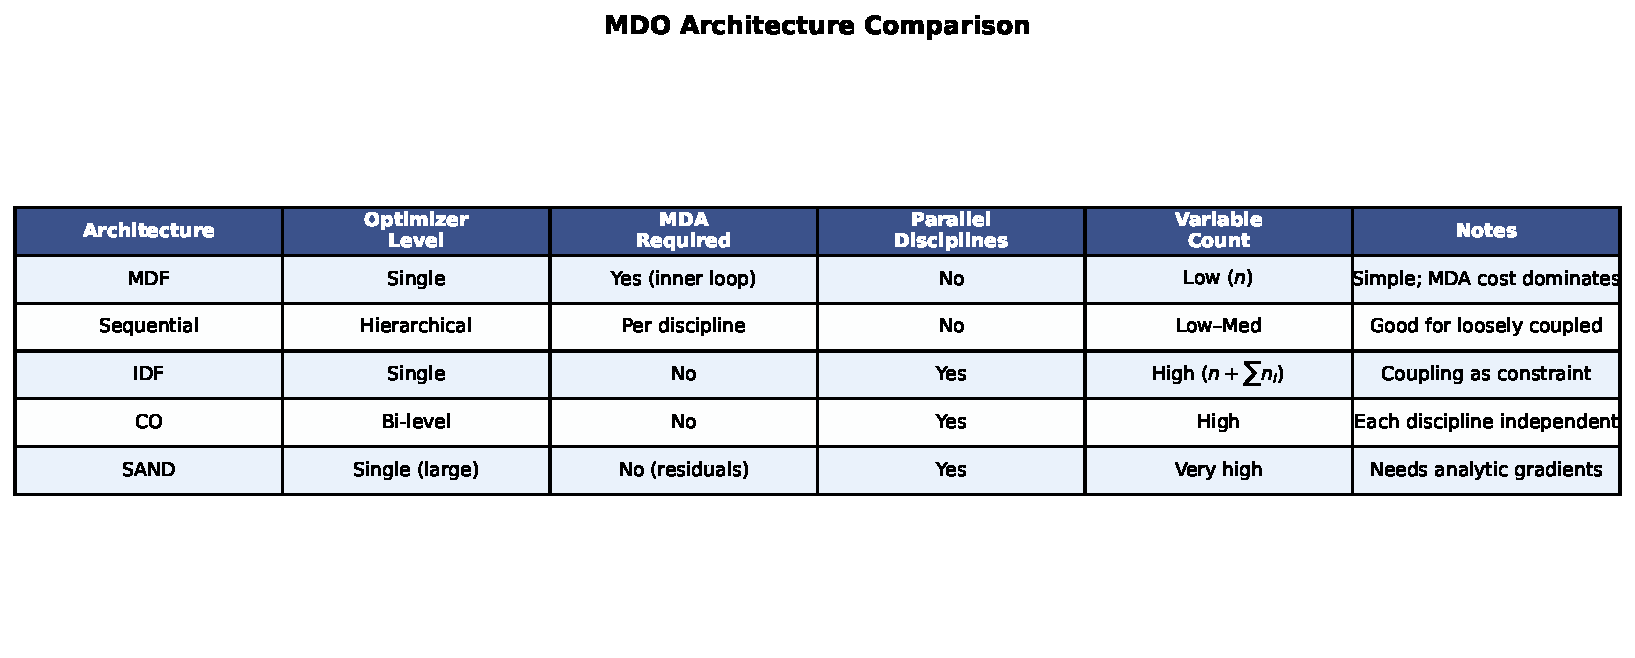
\includegraphics[width=0.72\textwidth]{fig_architecture_comparison.pdf}
  \end{center}

  \begin{columns}[T]
    \column{0.48\textwidth}
    \textbf{When to use each architecture:}

    \medskip
    \textit{Use MDF} when:
    \begin{itemize}
      \item The MDA converges in few iterations (loosely coupled system).
      \item You need physically feasible intermediates (e.g., for monitoring
            or early stopping).
      \item Disciplinary analyses are fast enough that the $K$-fold cost
            multiplier is acceptable.
      \item Black-box analyses without analytic derivatives.
    \end{itemize}

    \medskip
    \textit{Use IDF} when:
    \begin{itemize}
      \item The MDA is expensive (tightly coupled, many iterations).
      \item Disciplines can be parallelised.
      \item A gradient-based optimizer with constraint handling is available.
    \end{itemize}

    \column{0.48\textwidth}
    \textit{Use SAND} when:
    \begin{itemize}
      \item Analytic Jacobians (or an adjoint code) are available.
      \item The analysis code can be differentiated efficiently.
      \item Fastest wall-clock time is critical (e.g., real-time optimization).
    \end{itemize}

    \medskip
    \textit{Use CO} when:
    \begin{itemize}
      \item Different disciplines are owned by separate autonomous teams.
      \item Each team must use its own constraints and tools.
      \item Parallel execution of sub-problems is critical.
      \item The bi-level overhead is acceptable.
    \end{itemize}

    \medskip
    \textit{Use Sequential} when:
    \begin{itemize}
      \item Disciplines are loosely coupled.
      \item A modular round-robin approach suffices.
      \item Simplicity of implementation is prioritised over convergence guarantees.
    \end{itemize}
  \end{columns}

\end{frame}

% ============================================================================
\section{Summary}
% ============================================================================

\begin{frame}[allowframebreaks]{Chapter 24 Summary}

  This chapter has introduced the field of Multidisciplinary Design
  Optimization (MDO), the framework for optimising engineering systems
  in which multiple interacting analyses must be satisfied simultaneously.
  The following are the key ideas to carry away.

  \begin{block}{1. Assignments and Disciplinary Analyses}
    An assignment $\mathcal{A}$ collects all design variables
    $\mathbf{x}$ and response variables $\mathbf{y}^{(i)}$ into a single
    dictionary.  A disciplinary analysis $\mathcal{F}_i$ reads the current
    assignment and overwrites the response variables of discipline $i$.
    In the three-discipline running example:
    $y^{(1)} = y^{(2)} - x$, $y^{(2)} = \sin(y^{(1)} + y^{(3)})$,
    $y^{(3)} = \cos(x + y^{(1)} + y^{(2)})$.
  \end{block}

  \begin{block}{2. Interdisciplinary Compatibility and the MDA}
    An assignment is compatible if running any disciplinary analysis leaves
    it unchanged: $\mathcal{F}_i(\mathcal{A}) = \mathcal{A}$ for all $i$.
    The Gauss-Seidel MDA finds a compatible assignment iteratively.
    The ordering of analyses matters: a topologically sorted ordering
    converges faster and avoids oscillation.
  \end{block}

  \begin{block}{3. The Five MDO Architectures}
    All five architectures solve the same underlying problem --- minimise
    $f(\mathcal{A})$ subject to compatibility --- but differ in how they
    handle the coupling:
    \begin{enumerate}
      \item \textbf{MDF}: embed MDA inside the objective; optimizer sees
            a black box; every iterate is feasible.
      \item \textbf{Sequential}: round-robin discipline sub-problems;
            modular; no guarantee of system optimum.
      \item \textbf{IDF}: coupling copies in optimizer; equality constraints
            enforce compatibility; disciplines run in parallel.
      \item \textbf{CO}: bi-level; system optimizer sets targets; discipline
            sub-optimizers minimise coupling objectives.
      \item \textbf{SAND}: all variables free; residuals are constraints;
            no inner loops; requires analytic Jacobians.
    \end{enumerate}
  \end{block}

  \framebreak

  \begin{block}{4. The Spring-Pendulum Worked Example}
    The spring-pendulum system --- minimise spring stiffness $k$ subject to
    $\theta \leq 10^\circ$ --- concretely demonstrates all architectures.
    The MDA couples: $M = mg\ell\cos\theta$ (loads) and $\theta = M/k$
    (displacement).  All architectures converge to $k^* \approx 55.353$~N/m
    at $\theta^* = 10^\circ$ (the constraint boundary).
  \end{block}

  \begin{block}{5. Architectural Trade-offs}
    \begin{tabular}{@{}lcccc@{}}
      \toprule
      & Feasible & Parallel & Variable & Analytic \\
      Architecture & Iterates & Analyses & Space & Jac.\ Needed? \\
      \midrule
      MDF      & Yes & No  & Small  & No \\
      Sequential & Partial & Partial & Medium & No \\
      IDF      & No  & Yes & Large  & Helpful \\
      CO       & No  & Yes & Large (inner) & No \\
      SAND     & No  & Yes & Large  & Yes \\
      \bottomrule
    \end{tabular}
  \end{block}

  \begin{alertblock}{The Central Insight of MDO}
    There is no universally best architecture.  The right choice depends
    on the coupling strength (how much disciplines affect one another),
    the cost of individual analyses, the availability of derivatives,
    organisational structure, and whether feasible intermediates are required.
    Understanding these trade-offs is the practical core of MDO.
  \end{alertblock}

\end{frame}

% ============================================================================
\section{Exercises}
% ============================================================================

\begin{frame}[allowframebreaks]{Exercises}

  \begin{block}{Exercise 24.1: Real-World MDO Example}
    Provide an example of a real-world multidisciplinary design optimization
    problem involving at least three disciplines.  Draw the dependency
    diagram.  Identify which pairs of disciplines are \emph{tightly
    coupled} (strong circular dependency) and which are \emph{loosely
    coupled} (one-way or weak dependency).  Based on your dependency
    diagram, which MDO architecture would you recommend, and why?
  \end{block}

  \begin{block}{Exercise 24.2: Effect of Analysis Ordering}
    Consider the three-discipline system from Example 24.2:
    \[
      y^{(1)} = y^{(2)} - x, \quad
      y^{(2)} = \sin(y^{(1)} + y^{(3)}), \quad
      y^{(3)} = \cos(x + y^{(1)} + y^{(2)})
    \]
    Implement the Gauss-Seidel MDA in Python and run it for $x=1$ with
    (a) ordering $F_1, F_2, F_3$ and (b) ordering $F_1, F_3, F_2$.
    Plot the values of $y^{(1)}, y^{(2)}, y^{(3)}$ vs.\ iteration number
    for both orderings.  Explain, using the dependency graph, why one
    ordering converges and the other does not.
  \end{block}

  \begin{block}{Exercise 24.3: Topological Sorting}
    Given the ride-sharing dependency diagram (Vehicle $\to$ Sensor,
    Sensor $\to$ Vehicle (cycle), Sensor $\to$ Autonomy, Vehicle $\to$
    Autonomy, Autonomy $\to$ Routing, Routing $\to$ Demand (cycle),
    Demand $\to$ Routing, Demand $\to$ Profit, Routing $\to$ Profit):
    (a) Identify all strongly connected components (groups of disciplines
    that mutually depend on one another).
    (b) For each pair of tightly coupled analyses, what initial guess
    strategy would you use to start the MDA?
  \end{block}

  \framebreak

  \begin{block}{Exercise 24.4: Spring-Pendulum MDF}
    Formulate the spring-pendulum problem under the MDF architecture
    for $m = 1\,\mathrm{kg}$, $\ell = 1\,\mathrm{m}$,
    $g = 9.81\,\mathrm{m/s}^2$, $\theta_{\max} = 10^\circ$.
    Implement the MDA and the outer optimizer in Python using
    \texttt{scipy.optimize.minimize\_scalar}.
    Verify that $k^* \approx 55.353\,\mathrm{N/m}$ and that
    the constraint $\theta \leq \theta_{\max}$ is active at the
    optimum.  What does ``active constraint'' mean physically for
    the spring design?
  \end{block}

  \begin{block}{Exercise 24.5: Spring-Pendulum IDF}
    Reformulate the spring-pendulum problem under the IDF architecture.
    Identify the coupling variables (the optimizer-controlled copies of
    the response variables) and write down the two coupling equality
    constraints explicitly.
    Implement the IDF formulation in Python using
    \texttt{scipy.optimize.minimize} with \texttt{method='SLSQP'} and
    \texttt{NonlinearConstraint}.
    Verify that the IDF solution agrees with the MDF solution
    ($k^* \approx 55.353\,\mathrm{N/m}$) and that the coupling residuals
    are essentially zero at the solution.
  \end{block}

  \begin{block}{Exercise 24.6: Spring-Pendulum CO}
    Formulate the spring-pendulum problem under the Collaborative
    Optimization architecture.  Write out explicitly:
    (a) the displacement sub-problem (minimising $J_{\mathrm{disp}}$),
    (b) the loads sub-problem (minimising $J_{\mathrm{loads}}$), and
    (c) the system-level problem (minimise $k_g$ subject to $J^*_{\mathrm{disp}}=0$
    and $J^*_{\mathrm{loads}}=0$).
    What are the global variables $\mathcal{A}_g$?
    Discuss: what advantage does the CO decomposition offer if the
    loads team uses a proprietary finite-element solver and the
    structures team uses a proprietary stress-analysis code?
  \end{block}

\end{frame}

\begin{frame}{Further Reading and References}
  \begin{thebibliography}{9}
    \bibitem{kw2026}
    M.~J.\ Kochenderfer and T.~A.\ Wheeler,
    \textit{Algorithms for Optimization}, 2nd~ed.,
    MIT Press, 2026. (Chapter 24.)

    \bibitem{martins2013}
    J.~R.~R.~A.\ Martins and A.~B.\ Lambe,
    ``Multidisciplinary design optimization: A survey of architectures,''
    \textit{AIAA Journal}, 51(9):2049--2075, 2013.
    The authoritative survey paper on MDO architectures; highly recommended
    for practitioners.

    \bibitem{Cramer1994}
    E.~J.\ Cramer, J.~E.~Dennis, P.~D.\ Frank, R.~M.\ Lewis,
    and G.~R.\ Shubin,
    ``Problem formulation for multidisciplinary optimization,''
    \textit{SIAM Journal on Optimization}, 4(4):754--776, 1994.
    The original paper that formalised MDF, IDF, and SAND architectures.

    \bibitem{Braun1996}
    R.~D.\ Braun and I.~M.\ Kroo,
    ``Use of the collaborative optimization architecture for launch
    vehicle design,''
    \textit{AIAA/NASA 6th Symposium on Multidisciplinary Analysis
    and Optimization}, 1996.
    The paper that introduced and validated the CO architecture on a
    real aerospace design problem.

    \bibitem{Lambe2012}
    A.~B.\ Lambe and J.~R.~R.~A.\ Martins,
    ``Extensions to the design structure matrix for the description
    of multidisciplinary design, analysis, and optimization processes,''
    \textit{Structural and Multidisciplinary Optimization},
    46(2):273--284, 2012.
    Introduces the XDSM (Extended Design Structure Matrix) notation
    widely used to document MDO architectures.
  \end{thebibliography}
\end{frame}

\end{document}
